\subsection{Principal Component Analysis}
The PCA algorithm was implemented using the Matlab functions provided in the exercise document. Figure \ref{3_333} shows the mean of the whole data set as well as the first element and its corresponding reconstructed vector using different k components. Figure  \ref{eigenvqlues_plot} shows the eigenvalues of the components and the reconstruction error using different k values.
\bigbreak
Comparing figures in \ref{eigenvqlues_plot}, there exists a relation between the reconstruction error and the eigenvalues. This implies that the number of k components directly influence the quality of the reconstruction. This can be verified in figure  \ref{3_333}, the reconstructed image from k=1 to k=2 clearly shows an aggressive improvement.

\begin{figure}[!htbp]
\caption{Left: Image of the mean vector of the whole data set. Right: Image of the first element of the dataset with different reconstructions.}
\label{3_333}
\medbreak
\begin{tabular}{ccccccc}
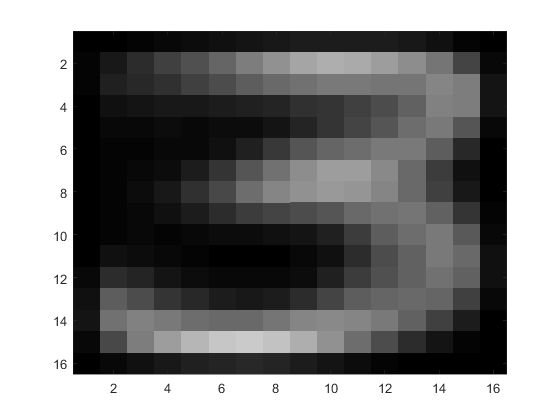
\includegraphics[width=\textwidth/7]{figures_3/mean_3} &
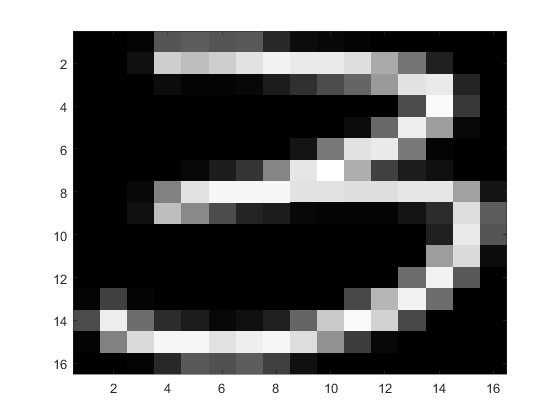
\includegraphics[width=\textwidth/7]{figures_3/k_0_1e} &
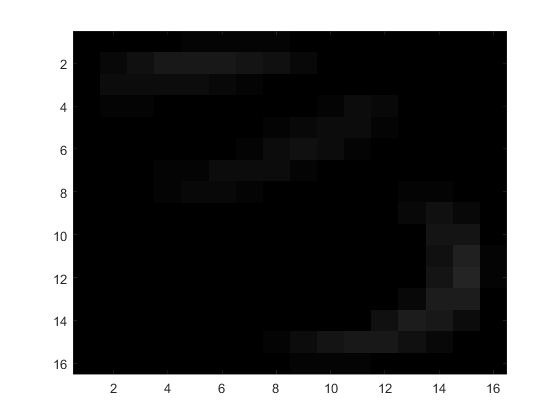
\includegraphics[width=\textwidth/7]{figures_3/k_1_1e} &
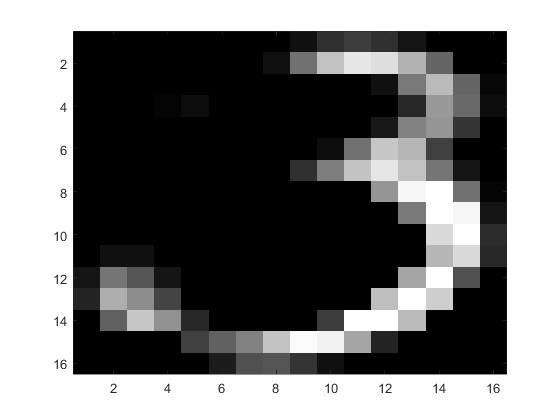
\includegraphics[width=\textwidth/7]{figures_3/k_2_1e} &
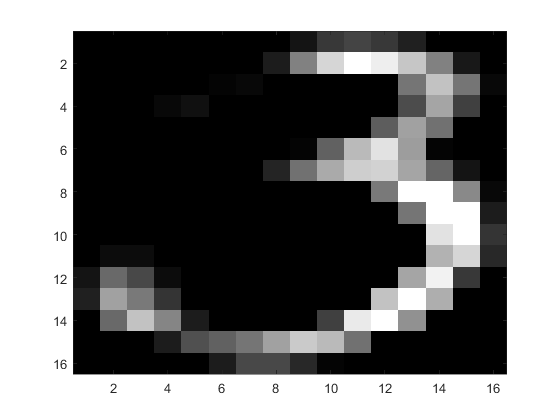
\includegraphics[width=\textwidth/7]{figures_3/k_3_1e} &
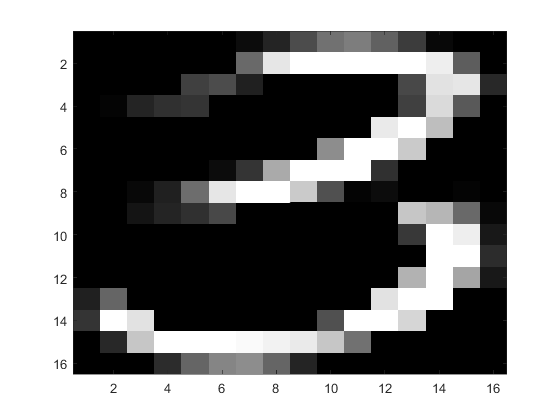
\includegraphics[width=\textwidth/7]{figures_3/k_4_1e}\\
 Mean & Original & k=1 & k=2 & k=3 & k=4\\
\end{tabular}
\centering
\end{figure}


\begin{figure}[!htbp]
\caption{Plots of PCA exercise.}
\label{eigenvqlues_plot}
  \centering
  \label{eigenvqlues_plot}
  \subfloat[Plot of the eigenvalues of the US Postal Service dataset. Axis X represents the \textit{i}th eigenvalue. Axis Y represents the eigenvalues.]{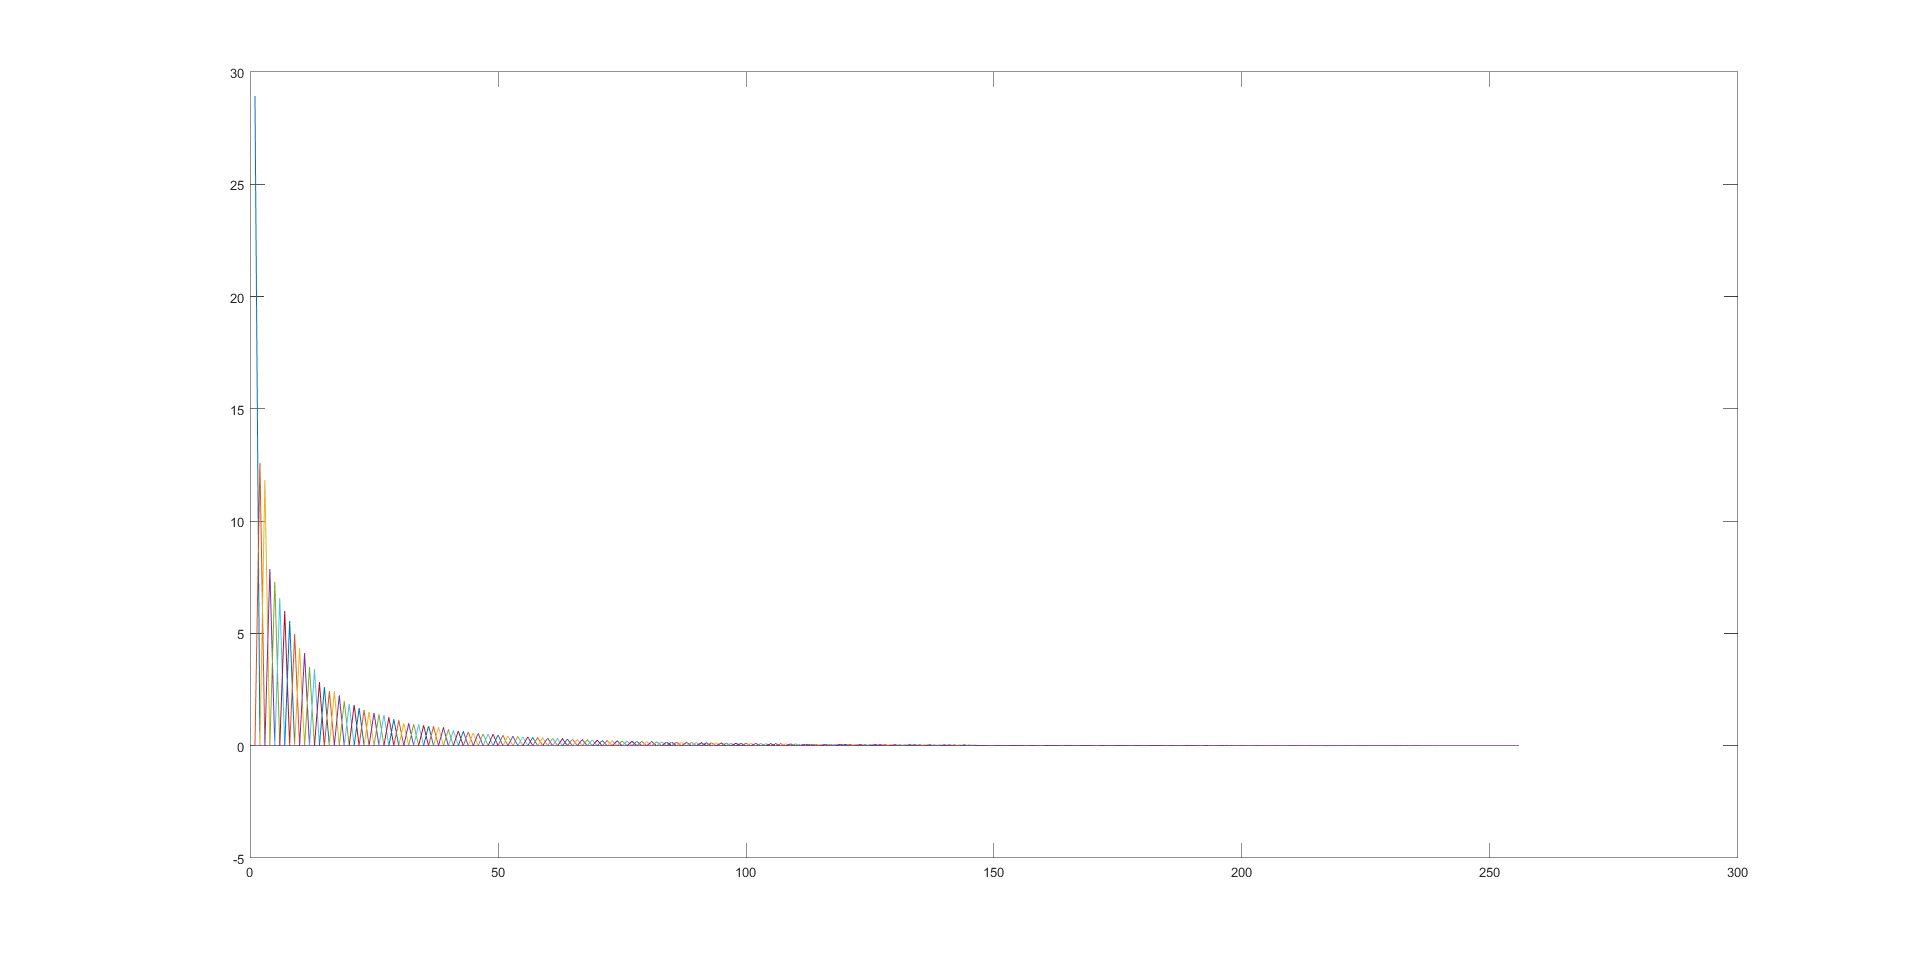
\includegraphics[width=0.4\textwidth]{figures_3/eigenvqlues_plot}\label{fig:f1}}
  \hfill
  \subfloat[Plot of the reconstructions error (MSE) from k=1 to k=256]{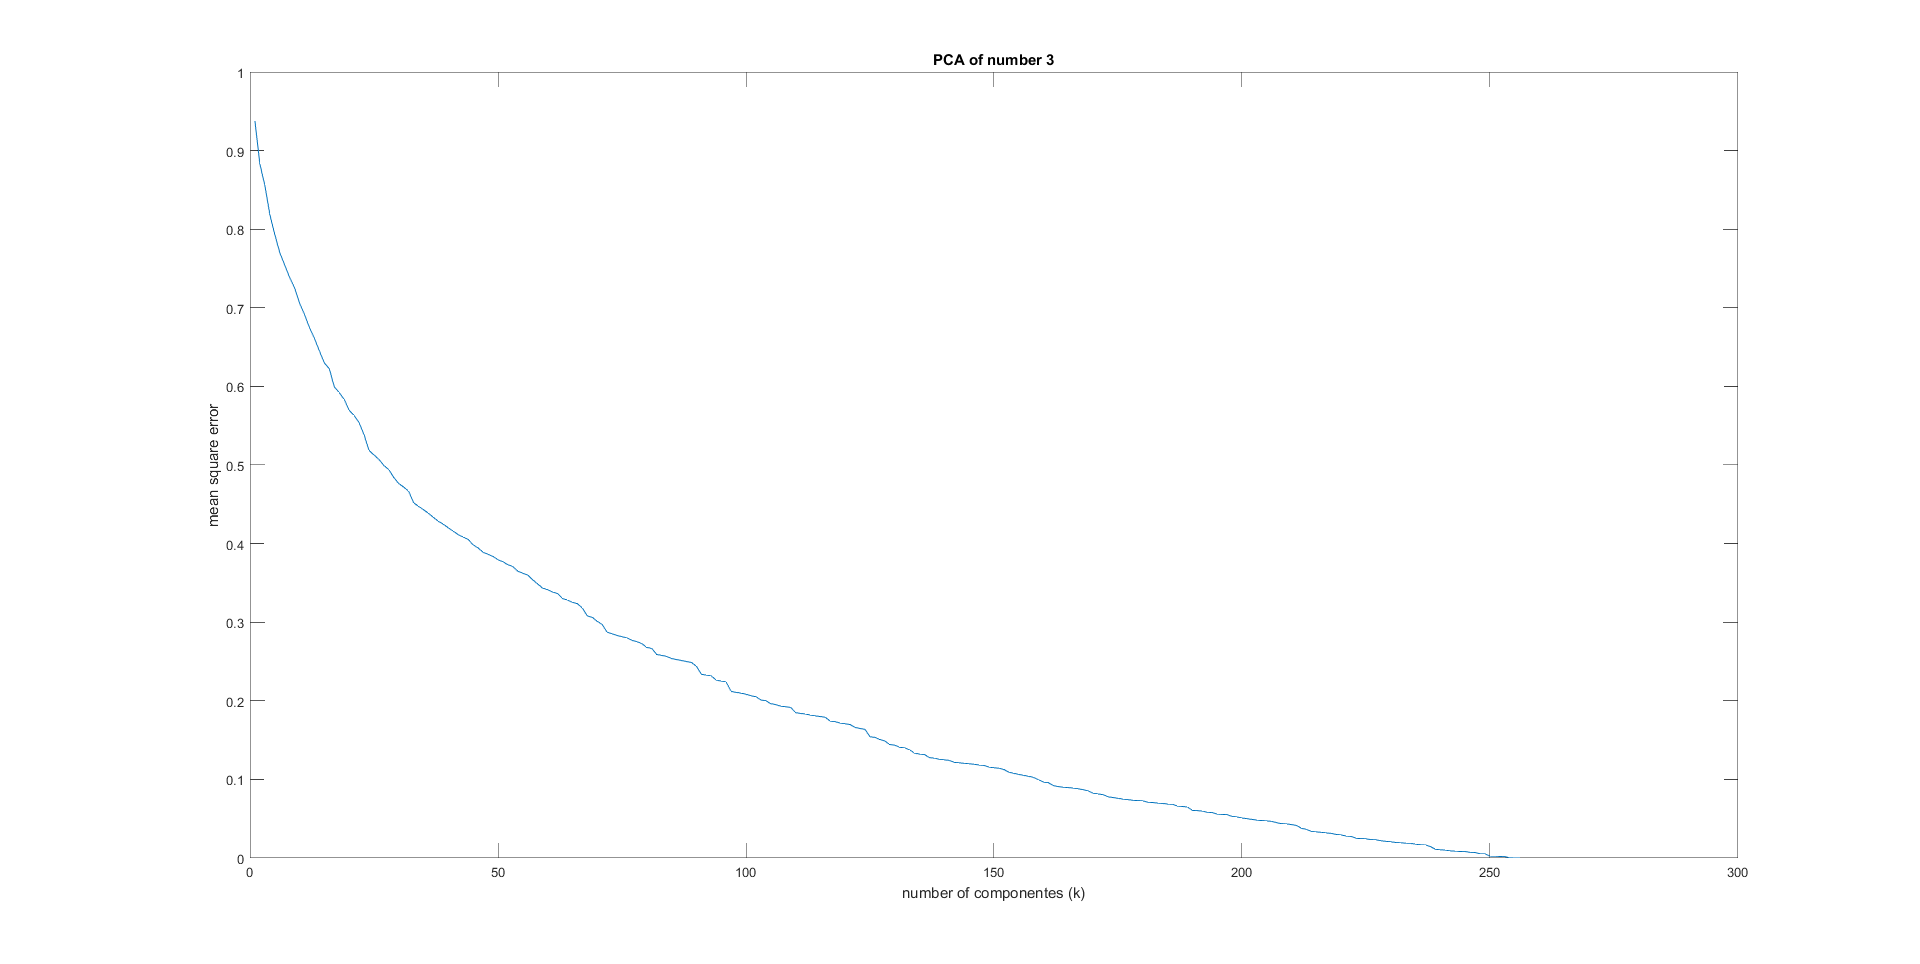
\includegraphics[width=0.4\textwidth]{figures_3/plot_k}\label{fig:f2}}
\end{figure}


\subsection{Competitive learning with SOM's}
Figure \ref{som_cylinder} shows the results of different experiment in \textbf{SOM\_concentric\_cylinders.m} script. The model used an hexagonal topology with a grid size of 5x5x5. \textit{Link distance} (linkdist) and \textit{Manhattan distance} (mandist) were tested with different epochs. 
\bigbreak
It is concluded that the \textit{linkdist} simulates a better cylinder shape (with a heavily connected graph) than the \textit{mandist}.
\bigbreak
\begin{figure}[!htbp]
\caption{Top: Trajectory of the neurons using Manhattan distance. Bottom: Trajectory of the neurons using Link distance.}
\label{som_cylinder}
\medbreak
\begin{tabular}{cccc}
 Initial state & epochs=10 & epochs=100 & epochs=1000\\\hline
 
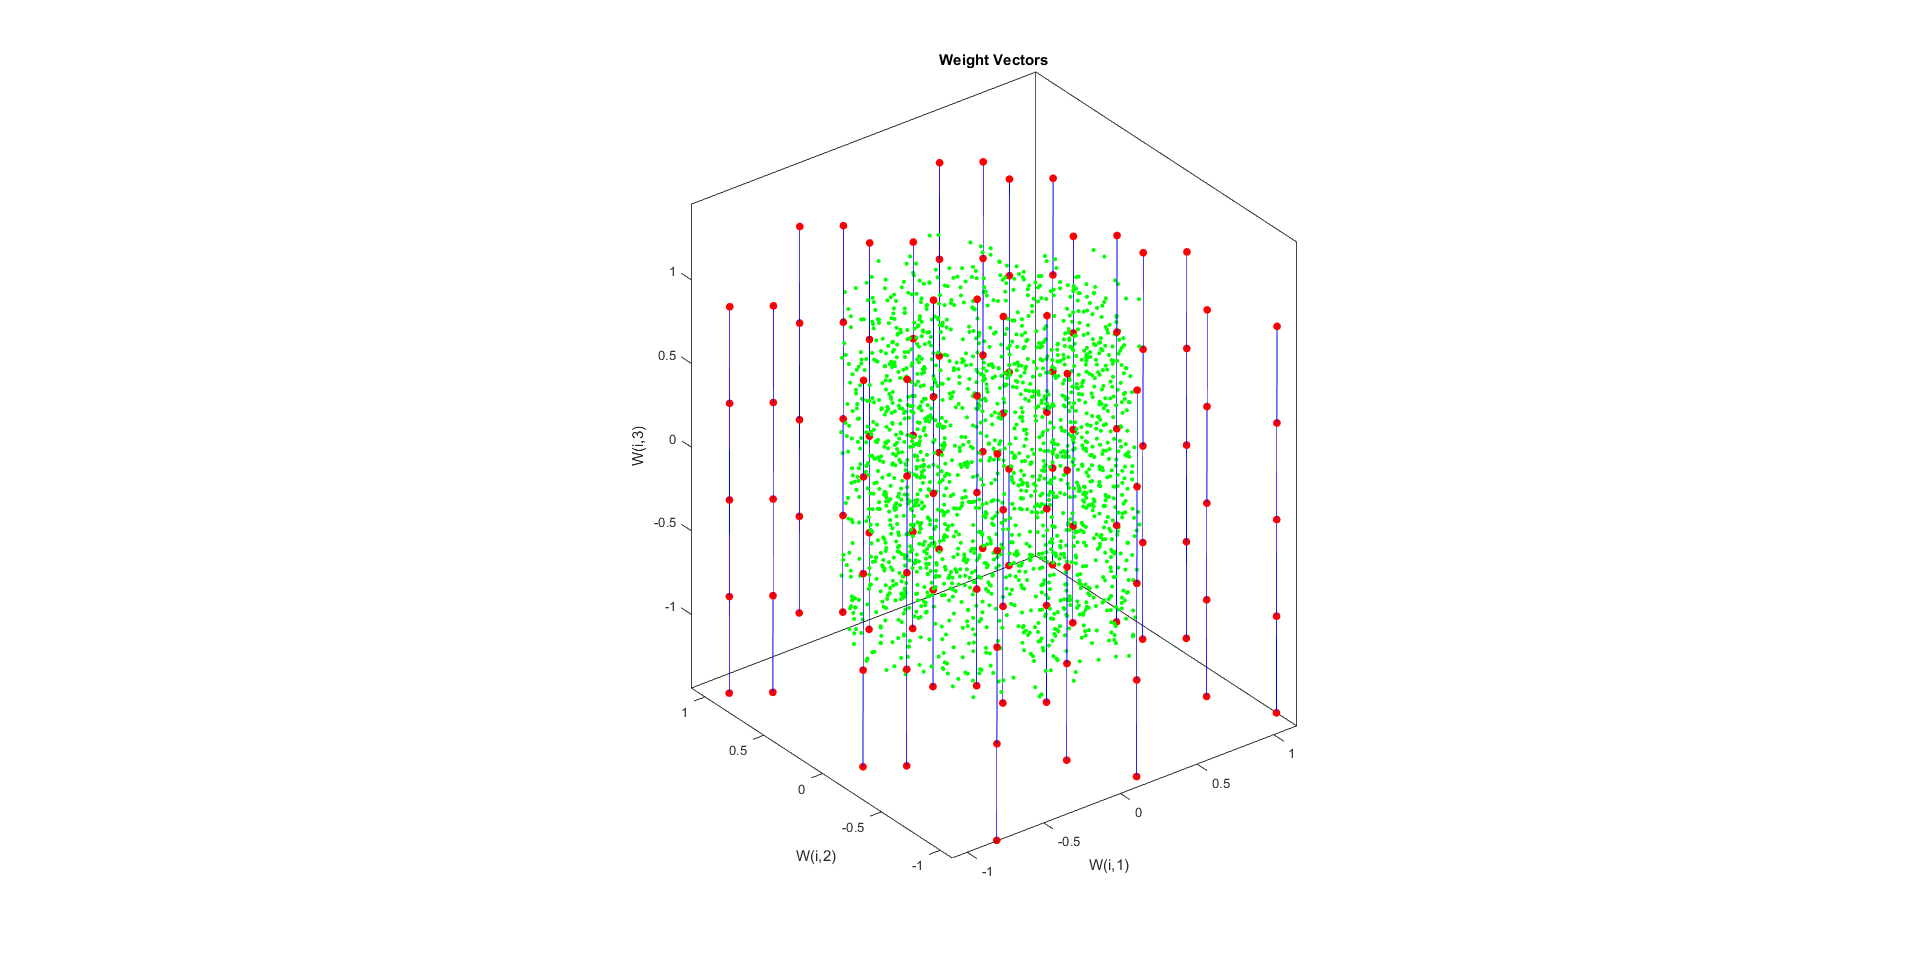
\includegraphics[width=\textwidth/5]{figures_3/som_0_1_mandist} &
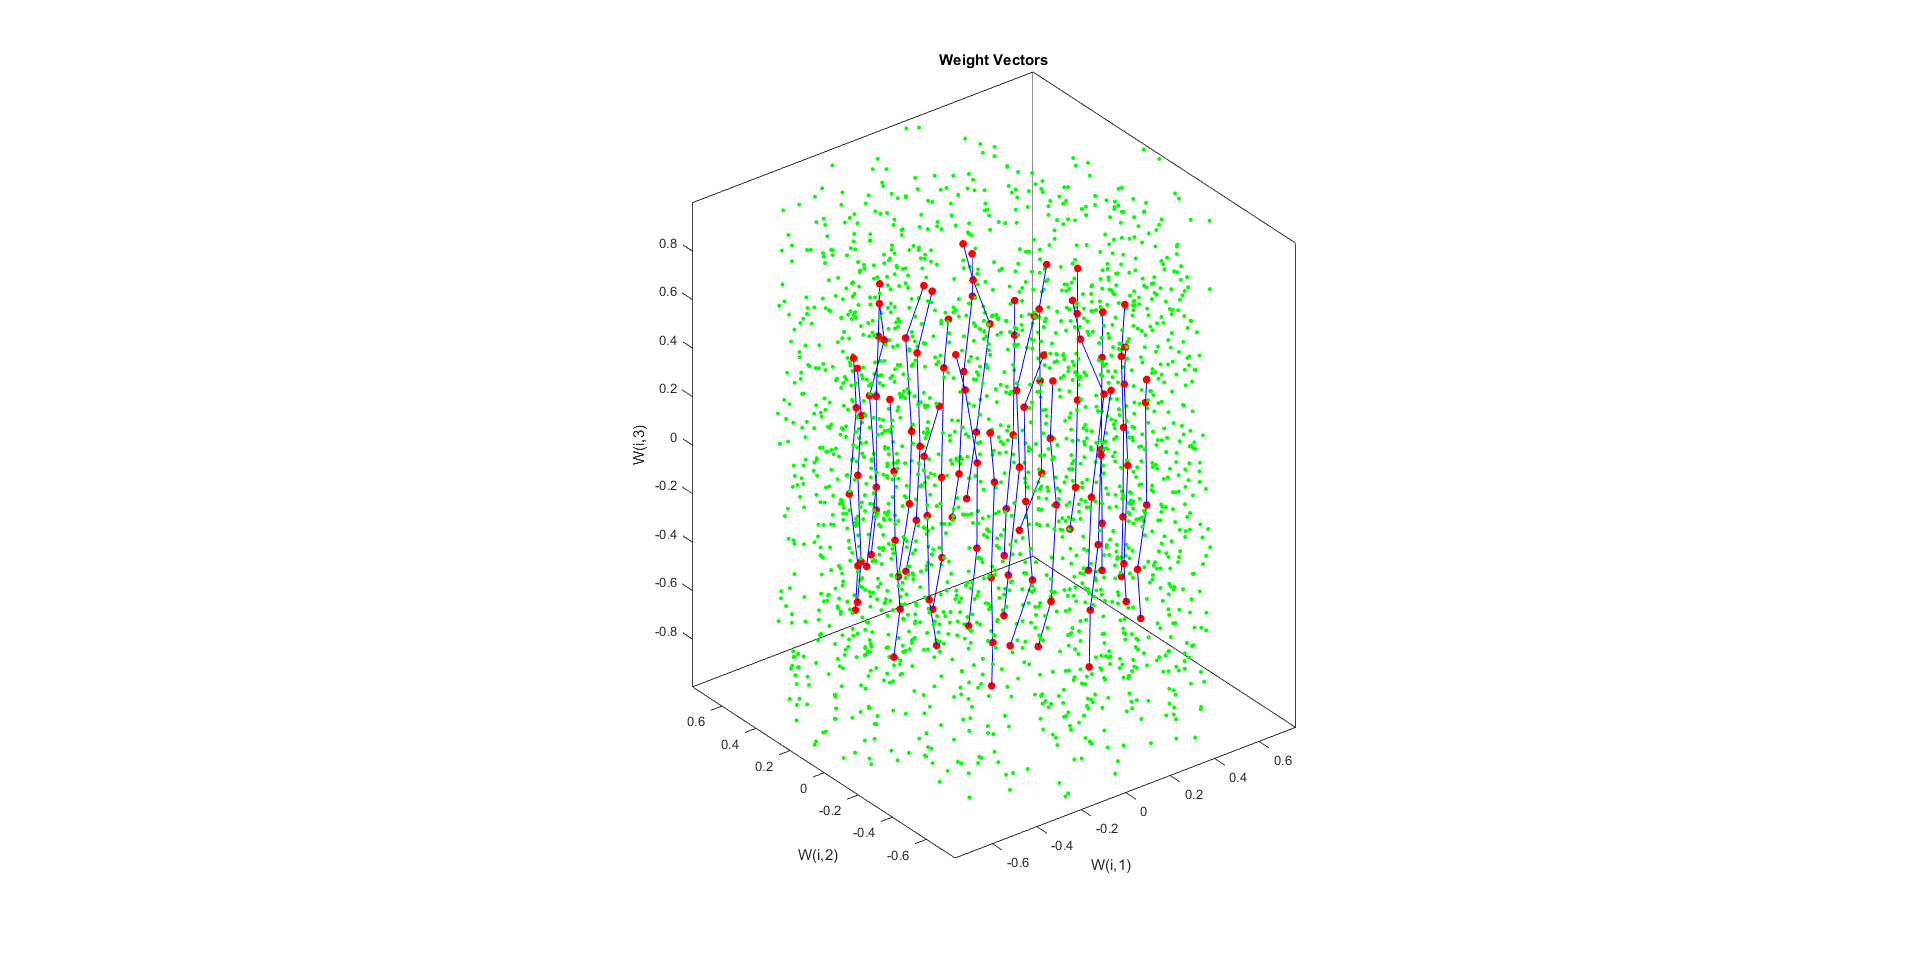
\includegraphics[width=\textwidth/5]{figures_3/som_10_1_mandist} &
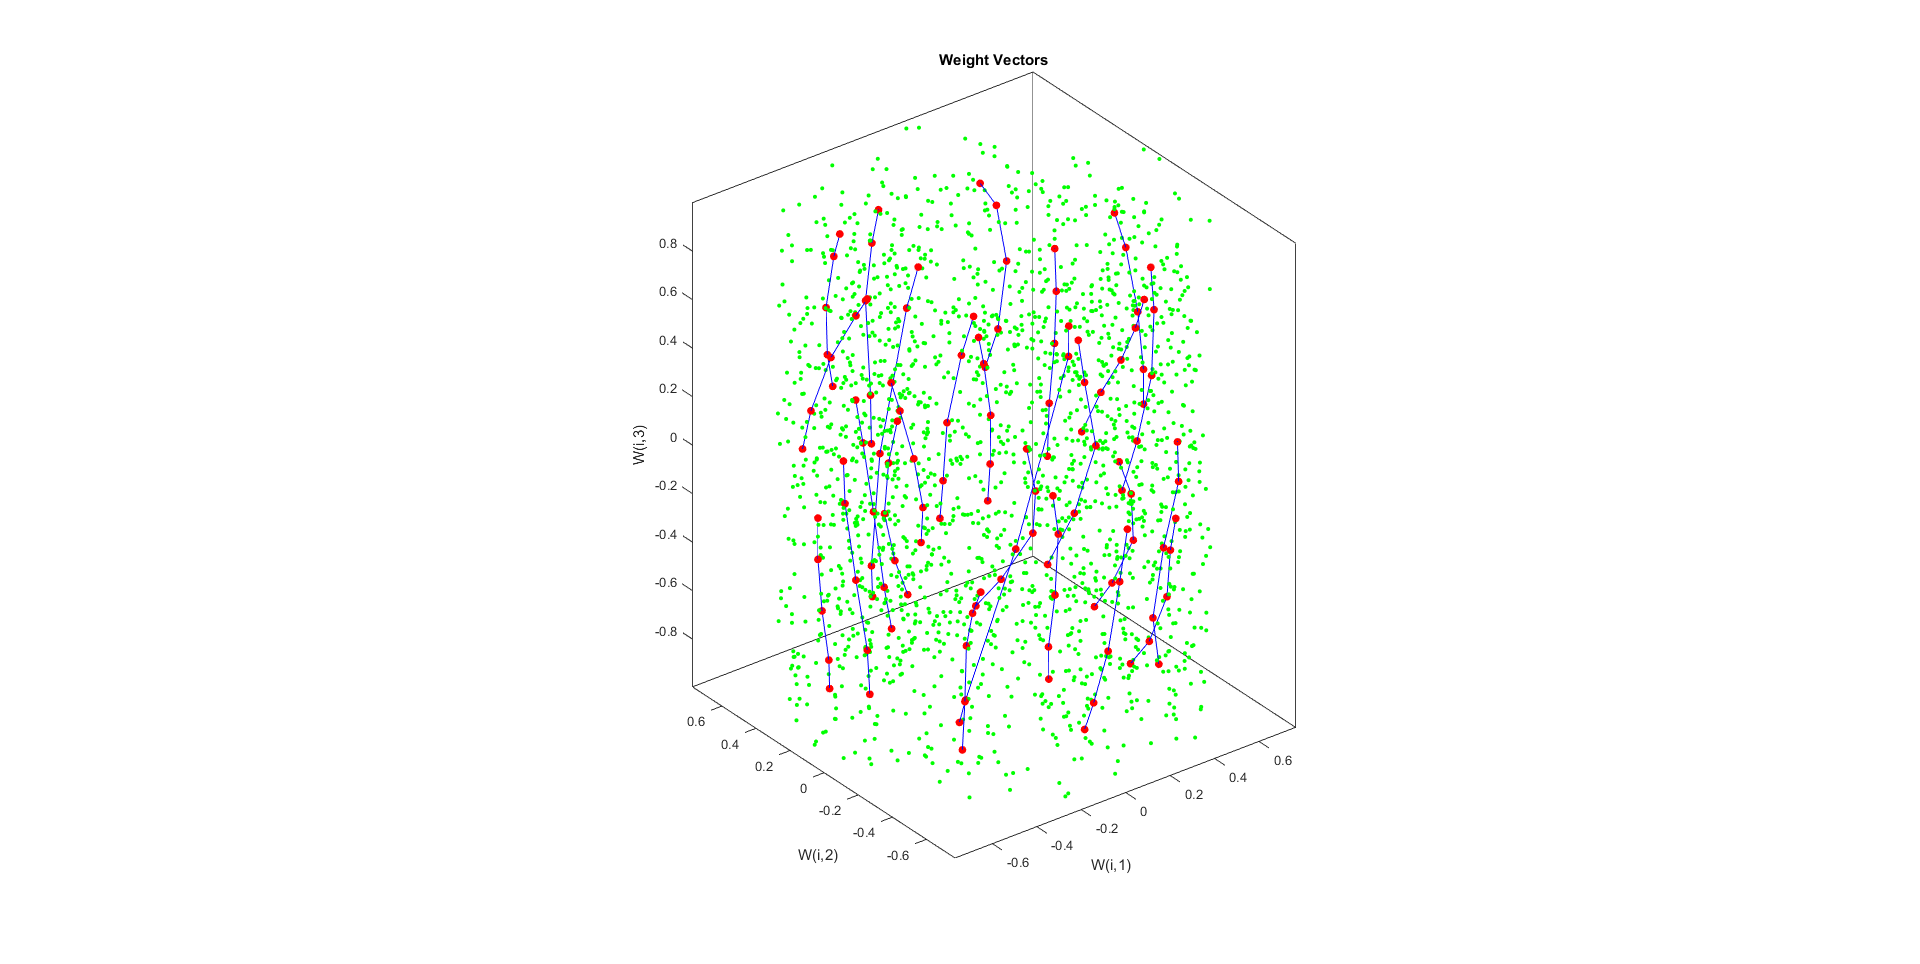
\includegraphics[width=\textwidth/5]{figures_3/som_100_1_mandist} &
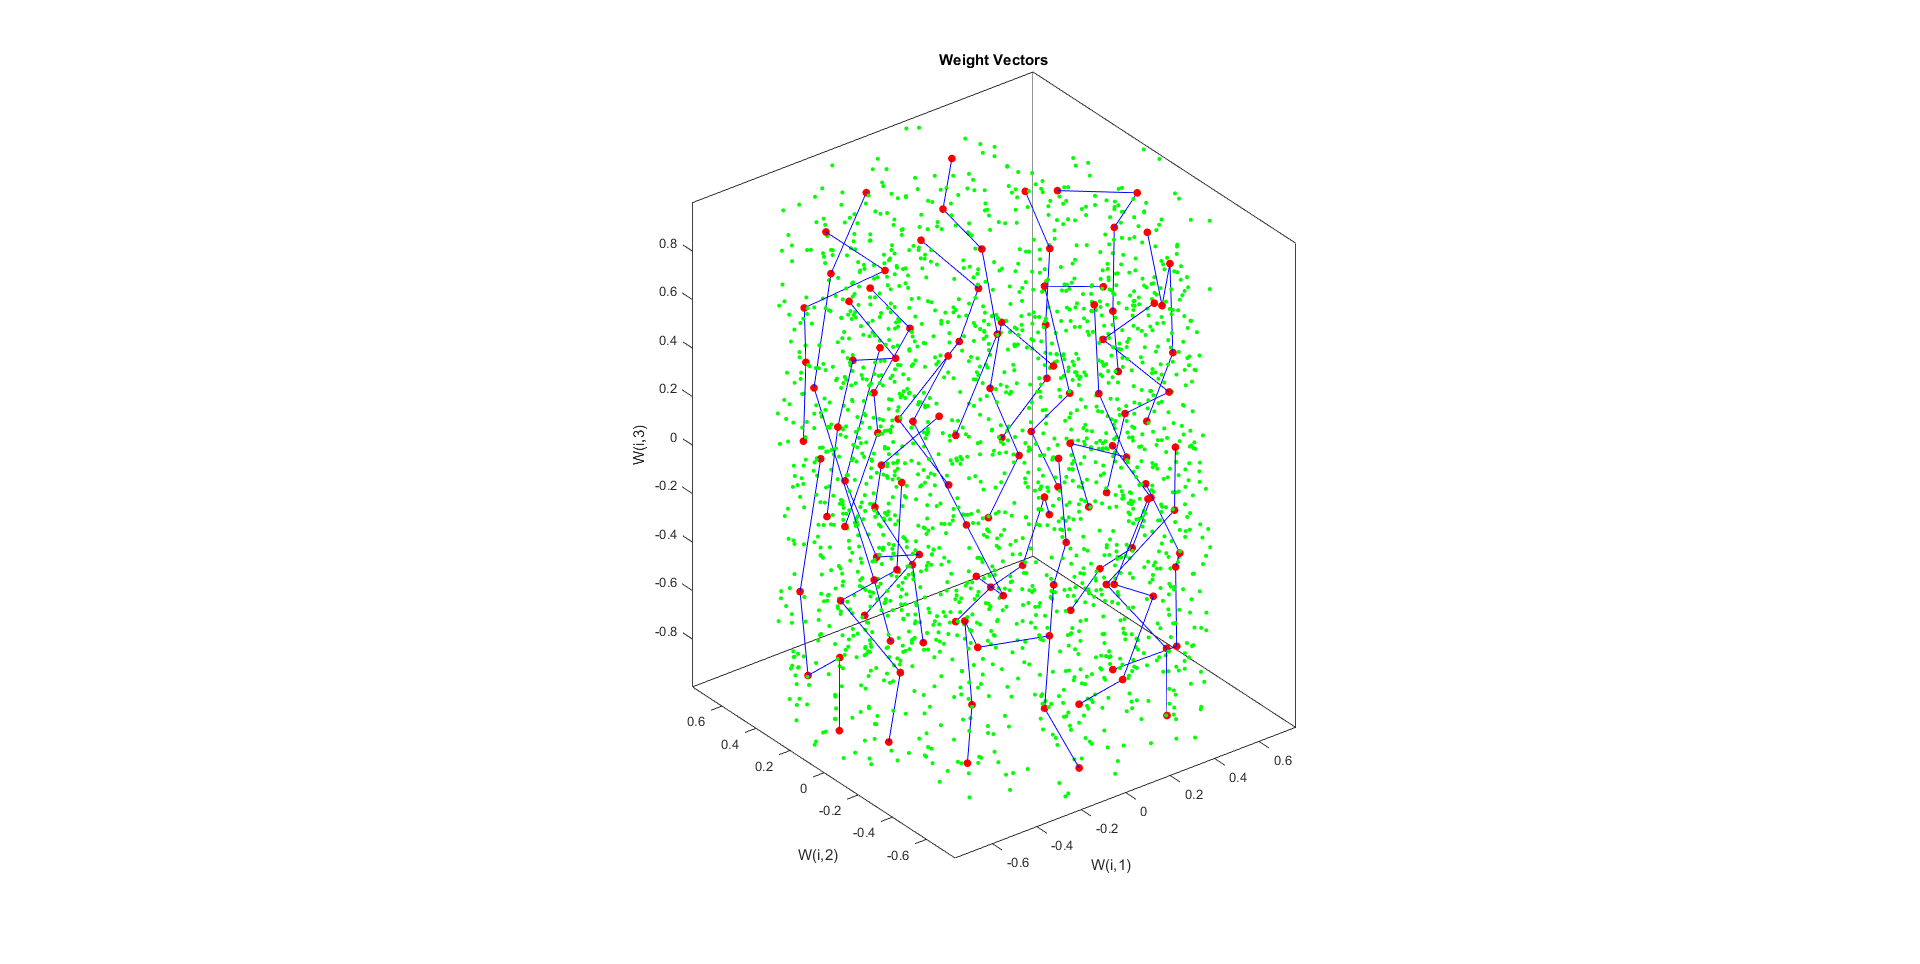
\includegraphics[width=\textwidth/5]{figures_3/som_1000_1_mandist} \\
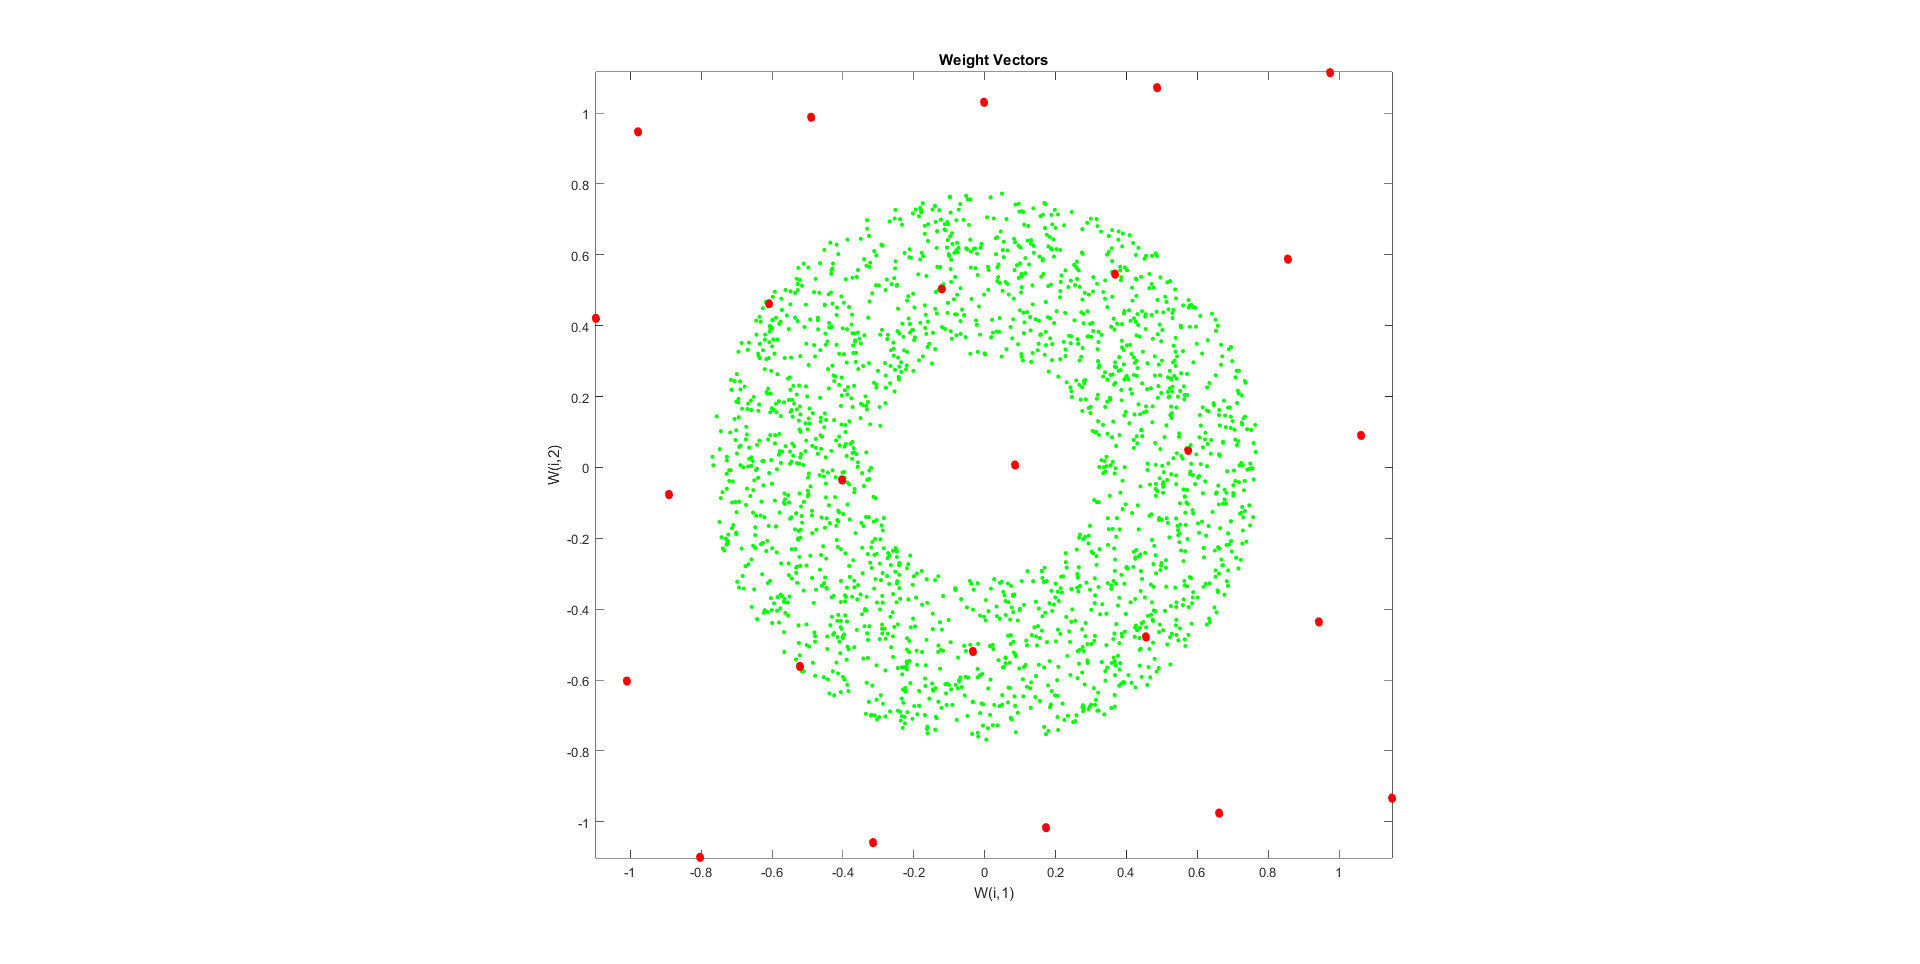
\includegraphics[width=\textwidth/5]{figures_3/som_0_2_mandist} &
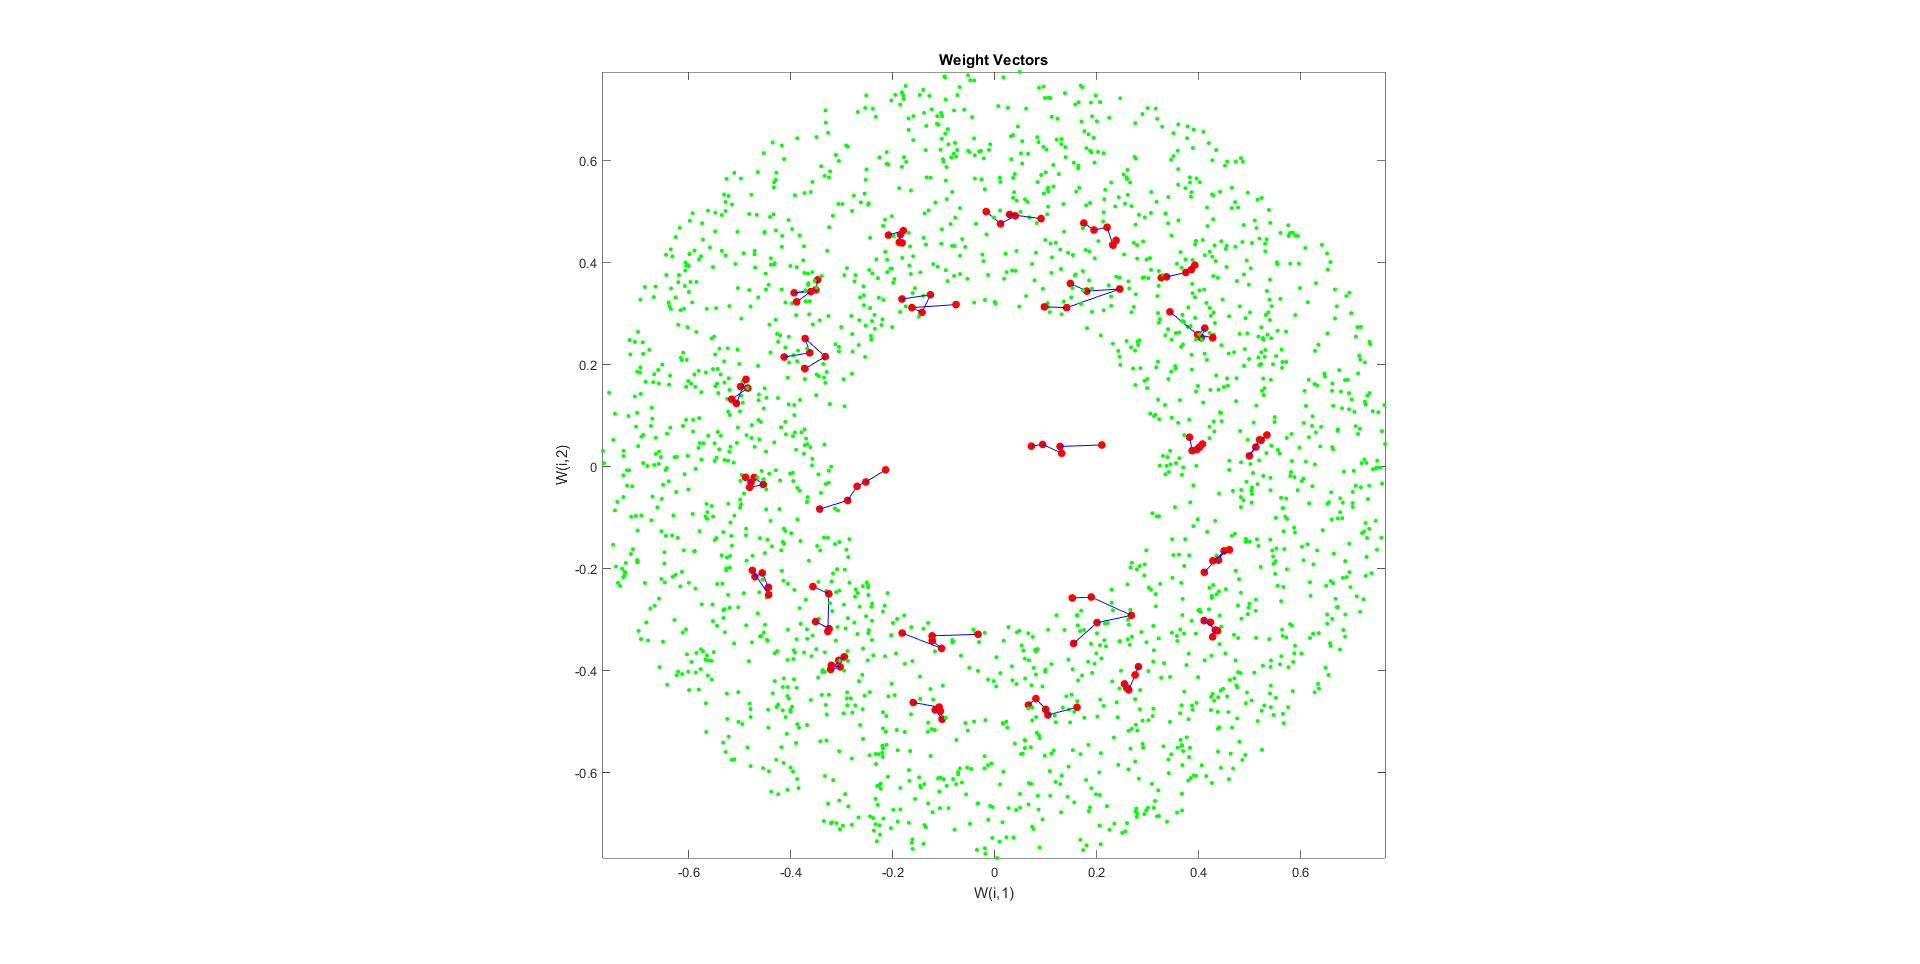
\includegraphics[width=\textwidth/5]{figures_3/som_10_2_mandist} &
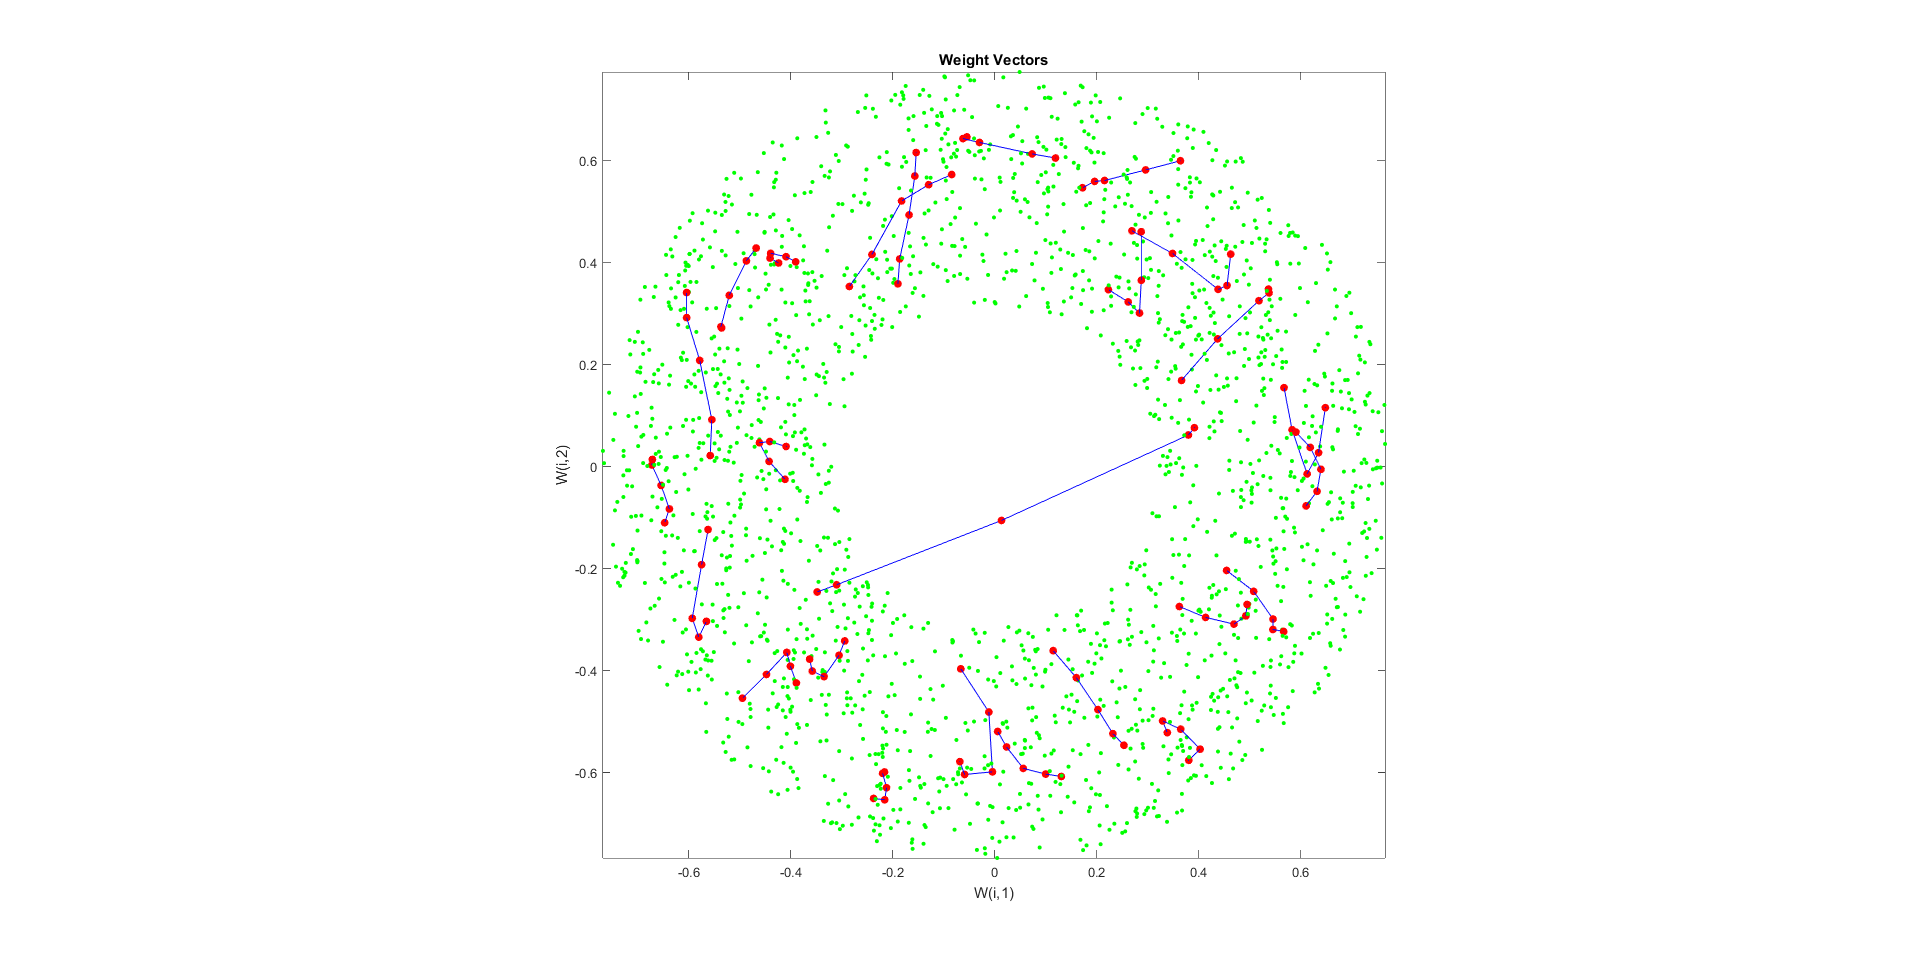
\includegraphics[width=\textwidth/5]{figures_3/som_100_2_mandist} &
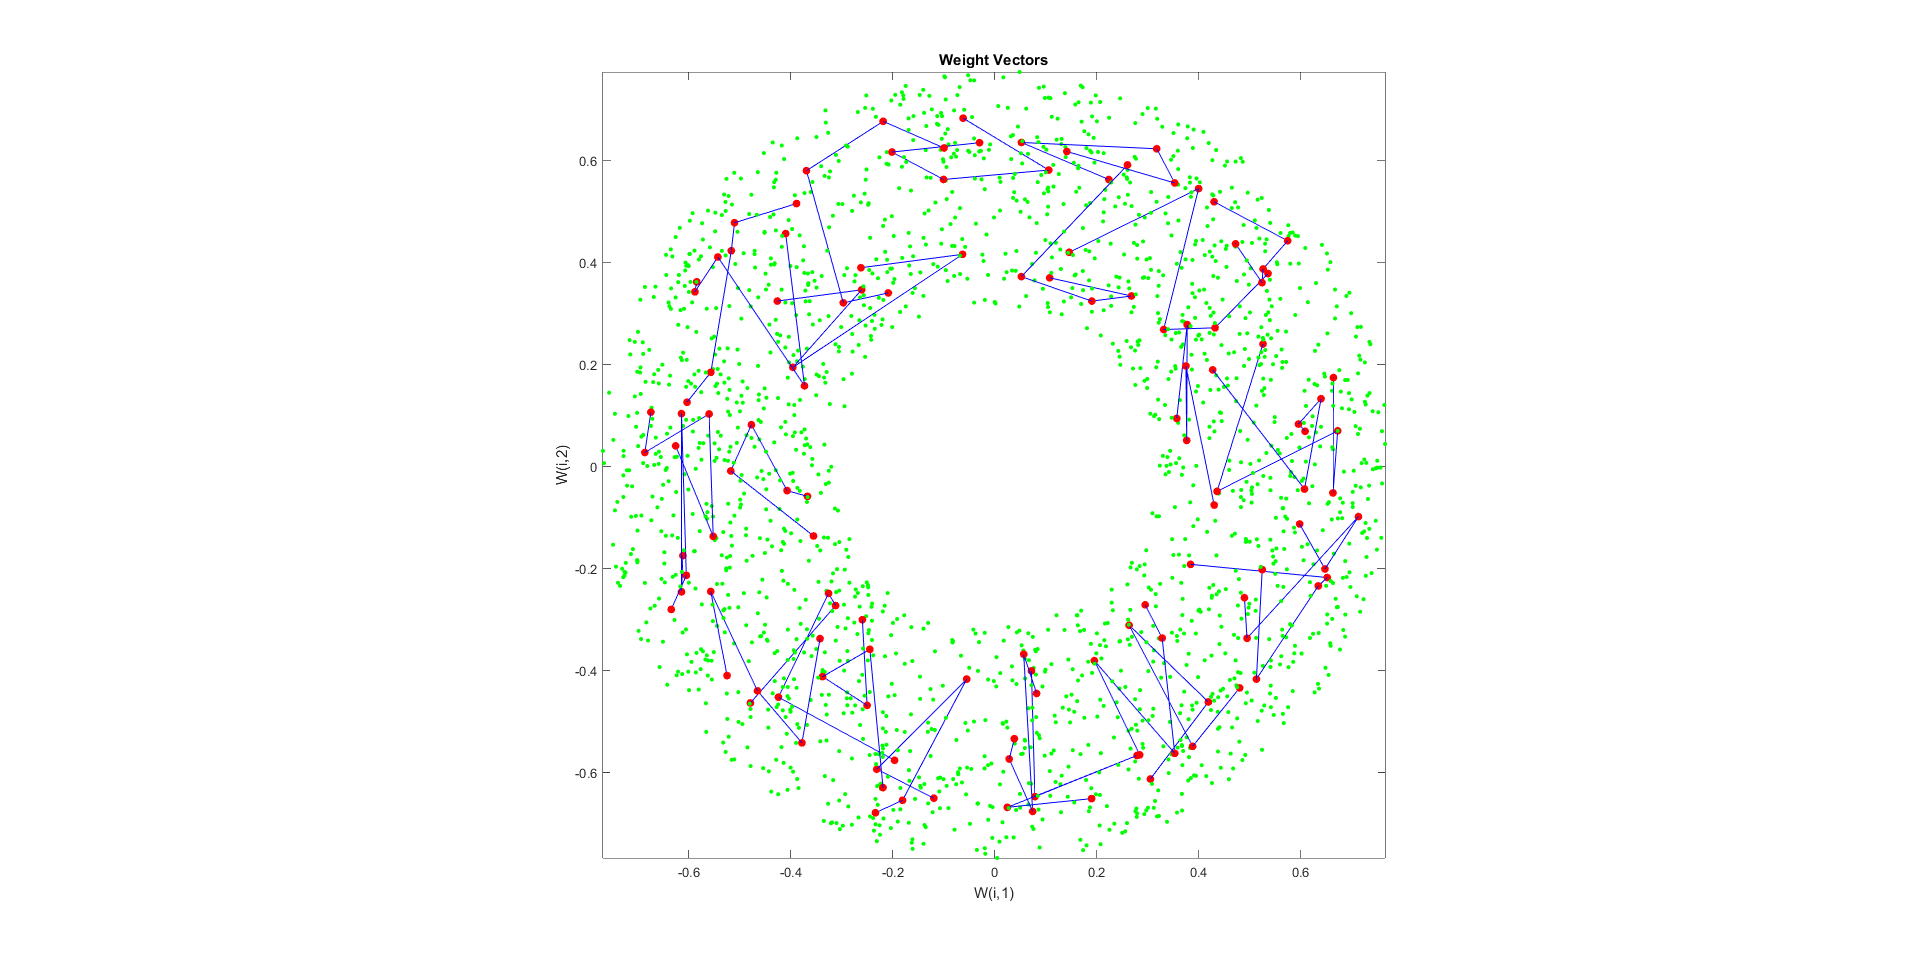
\includegraphics[width=\textwidth/5]{figures_3/som_1000_2_mandist} \\\hline

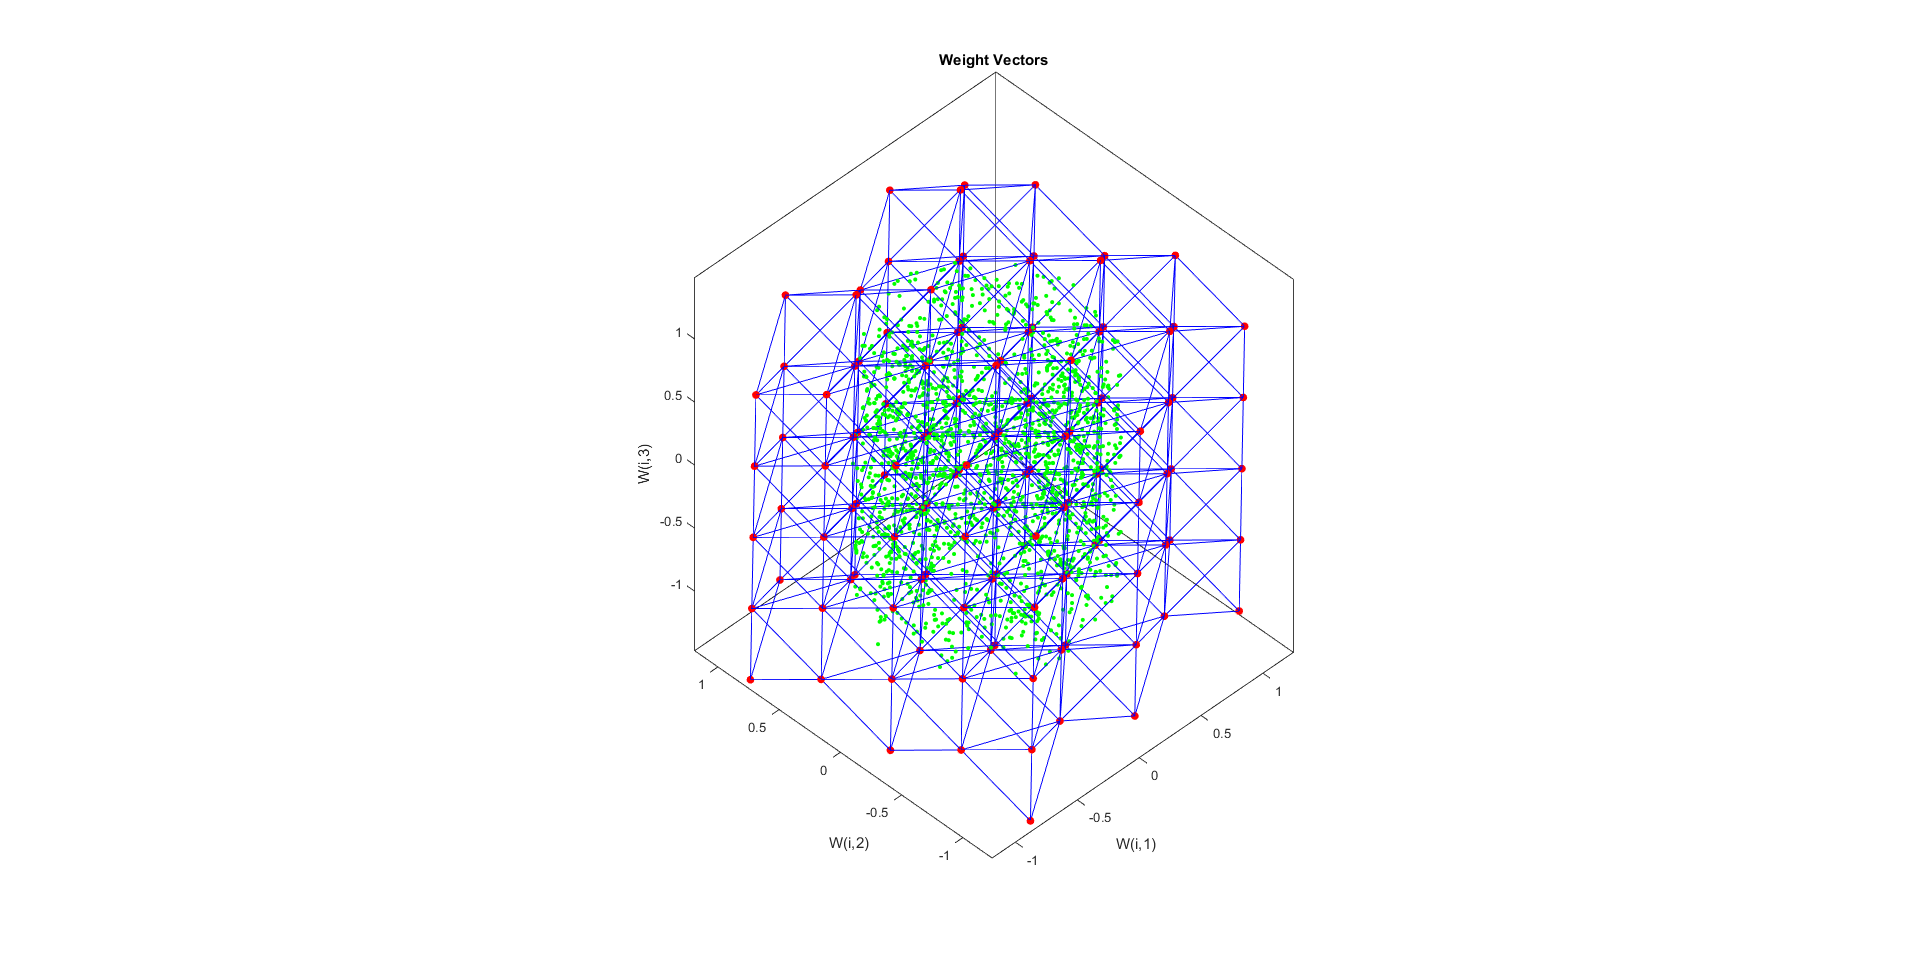
\includegraphics[width=\textwidth/5]{figures_3/som_0_1} &
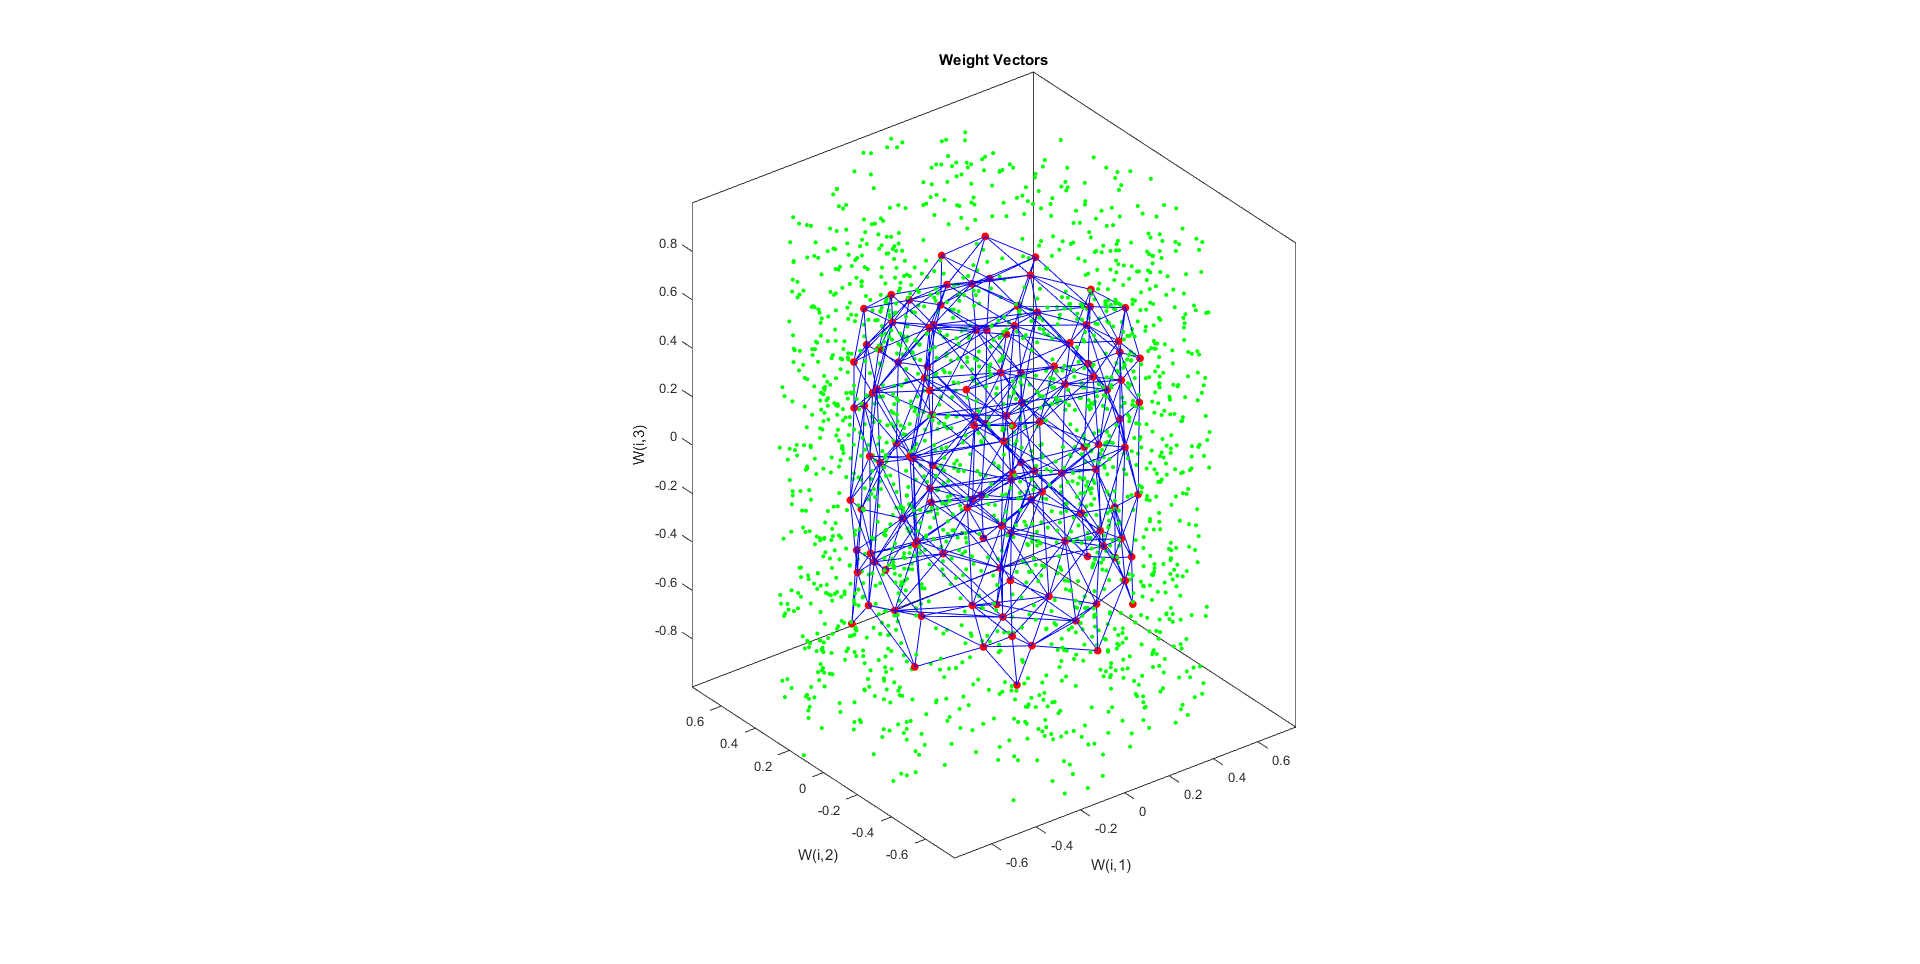
\includegraphics[width=\textwidth/5]{figures_3/som_10_1} &
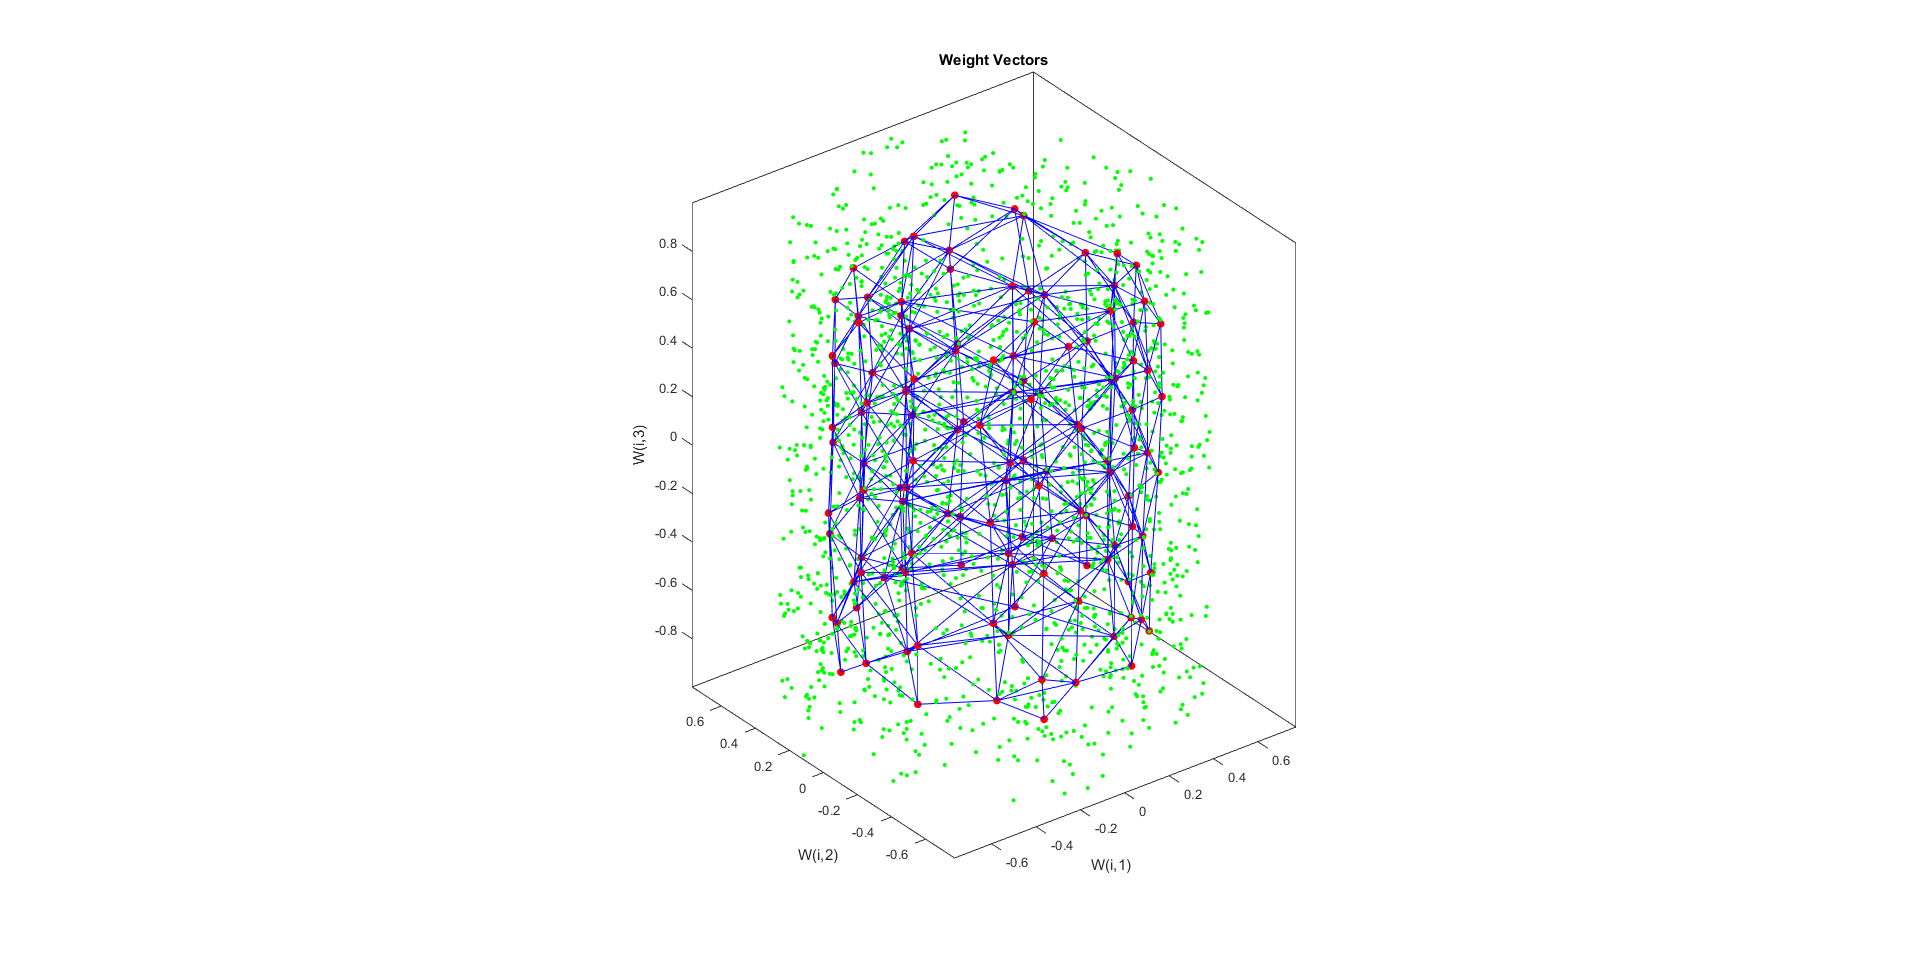
\includegraphics[width=\textwidth/5]{figures_3/som_100_1} &
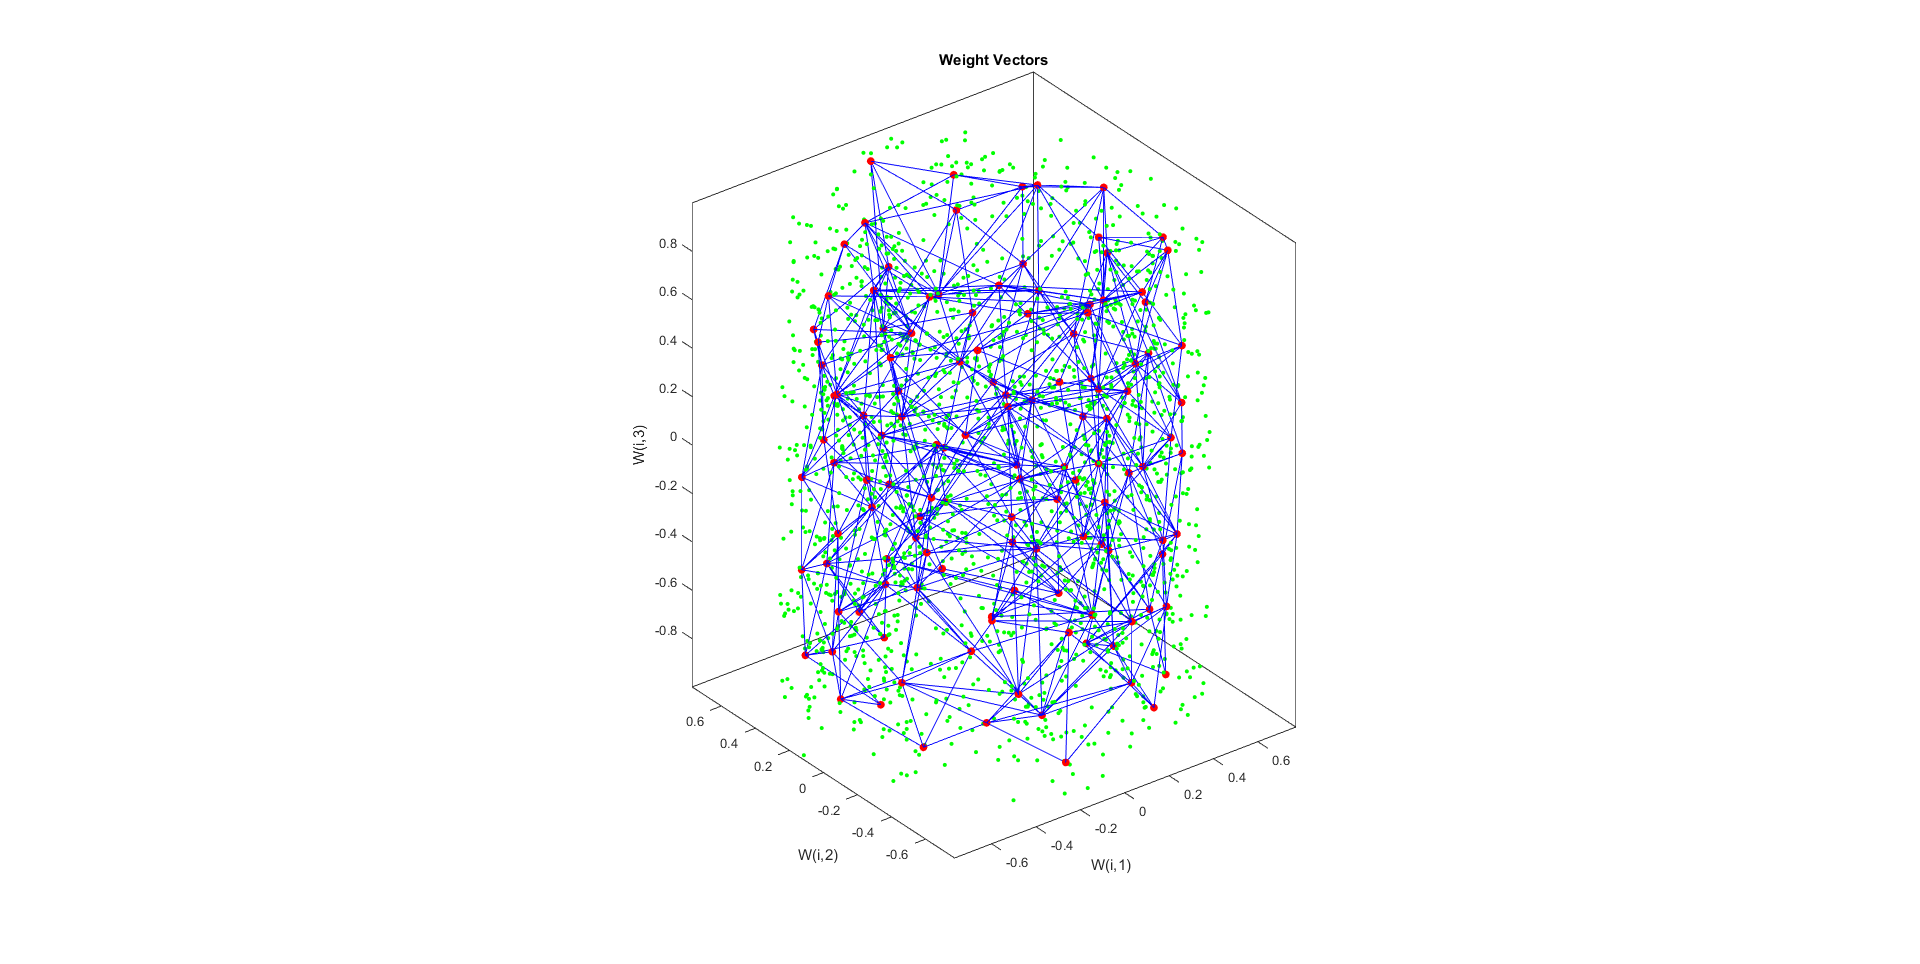
\includegraphics[width=\textwidth/5]{figures_3/som_1000_1} \\
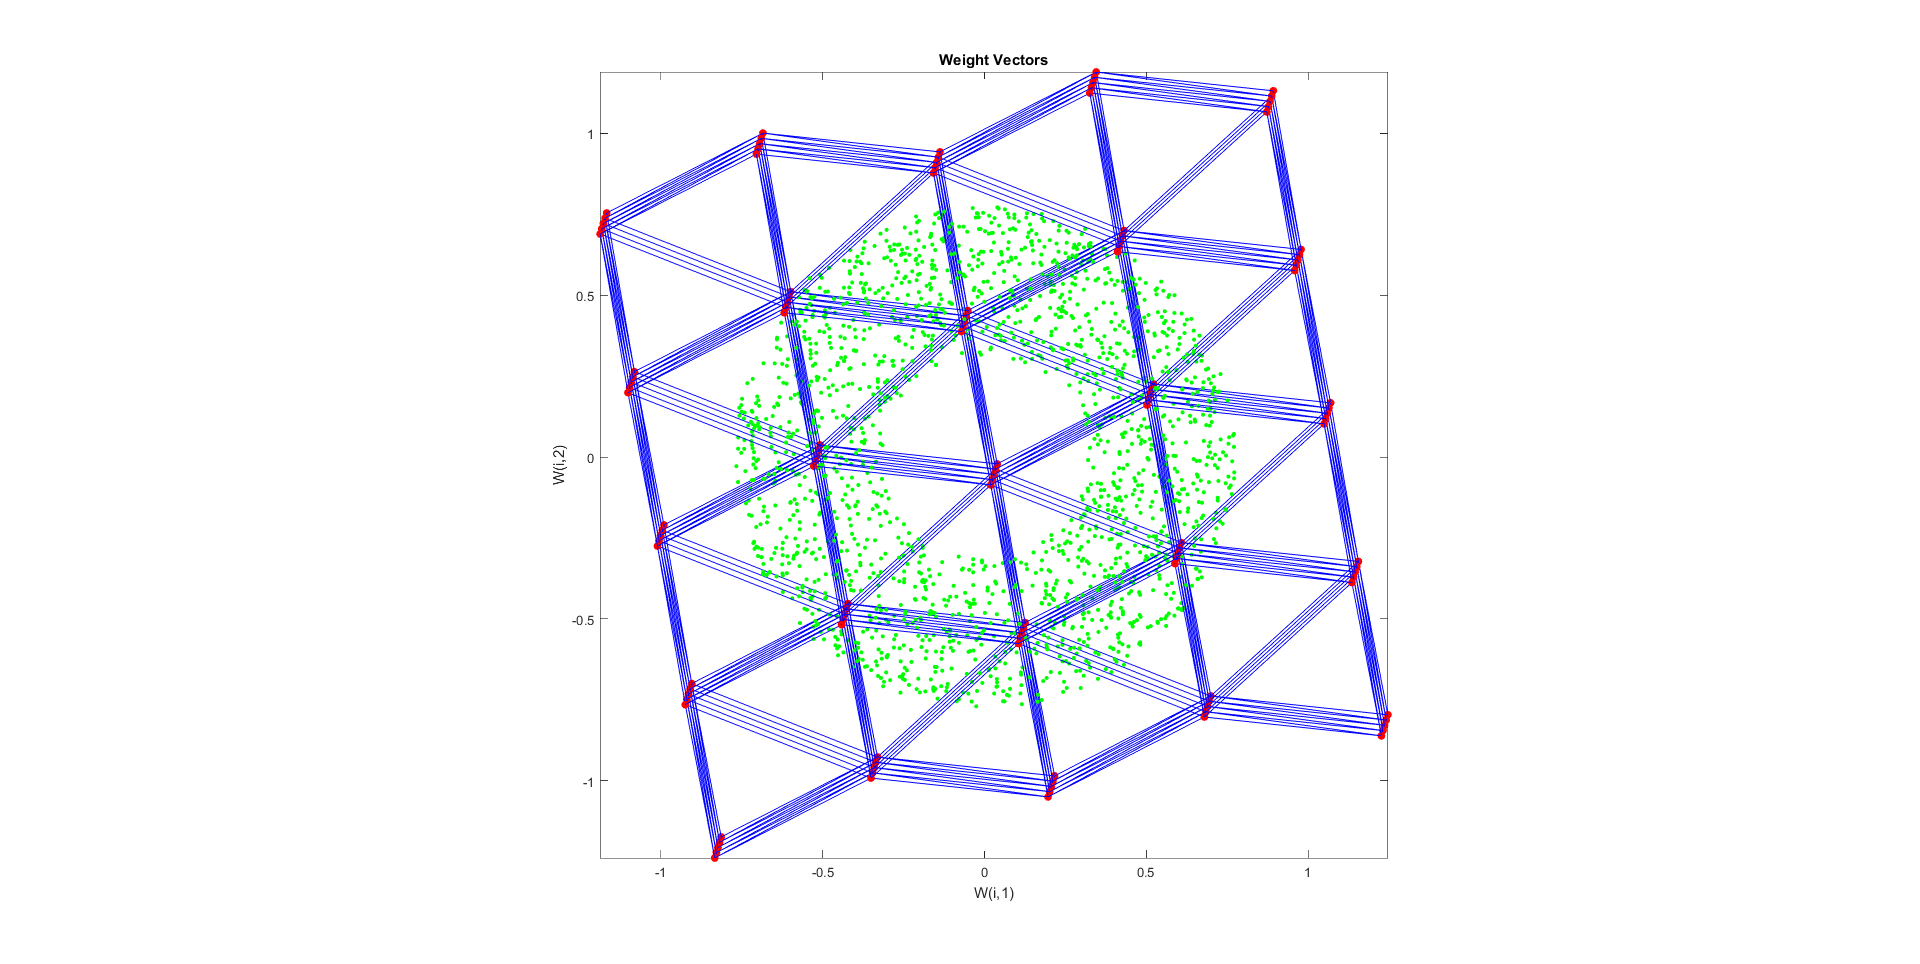
\includegraphics[width=\textwidth/5]{figures_3/som_0_2} &
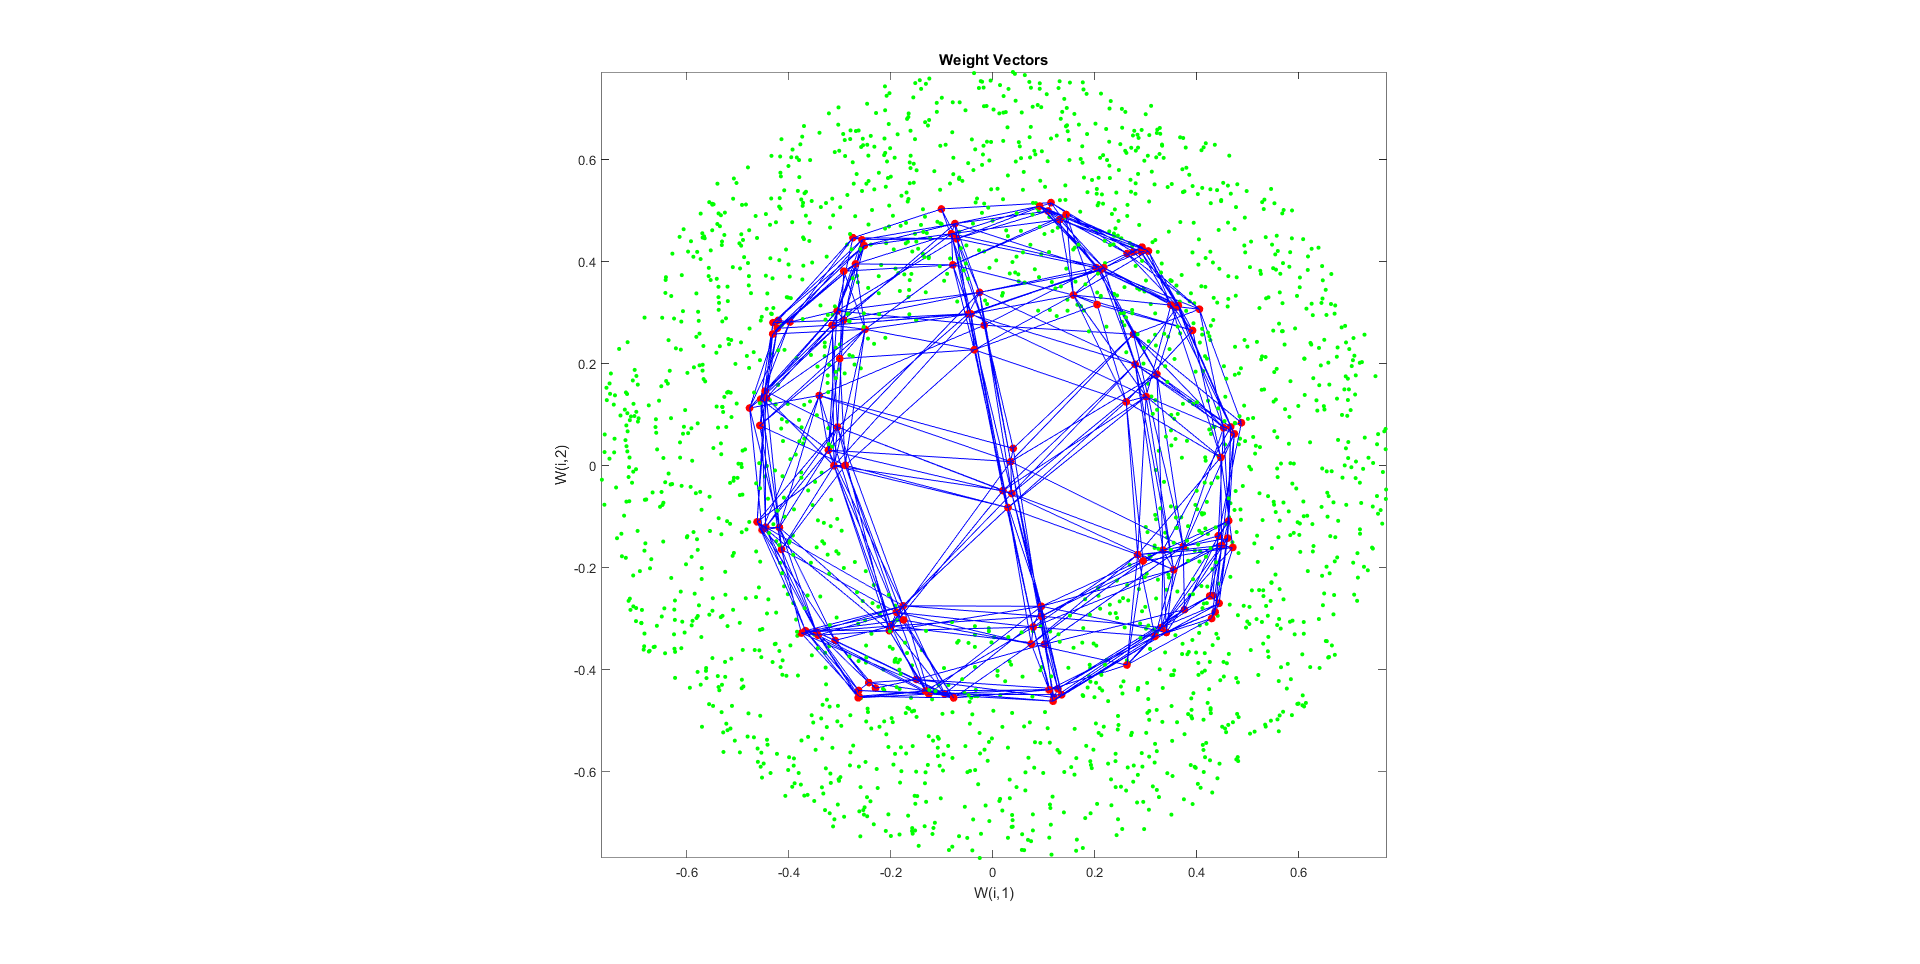
\includegraphics[width=\textwidth/5]{figures_3/som_10_2} &
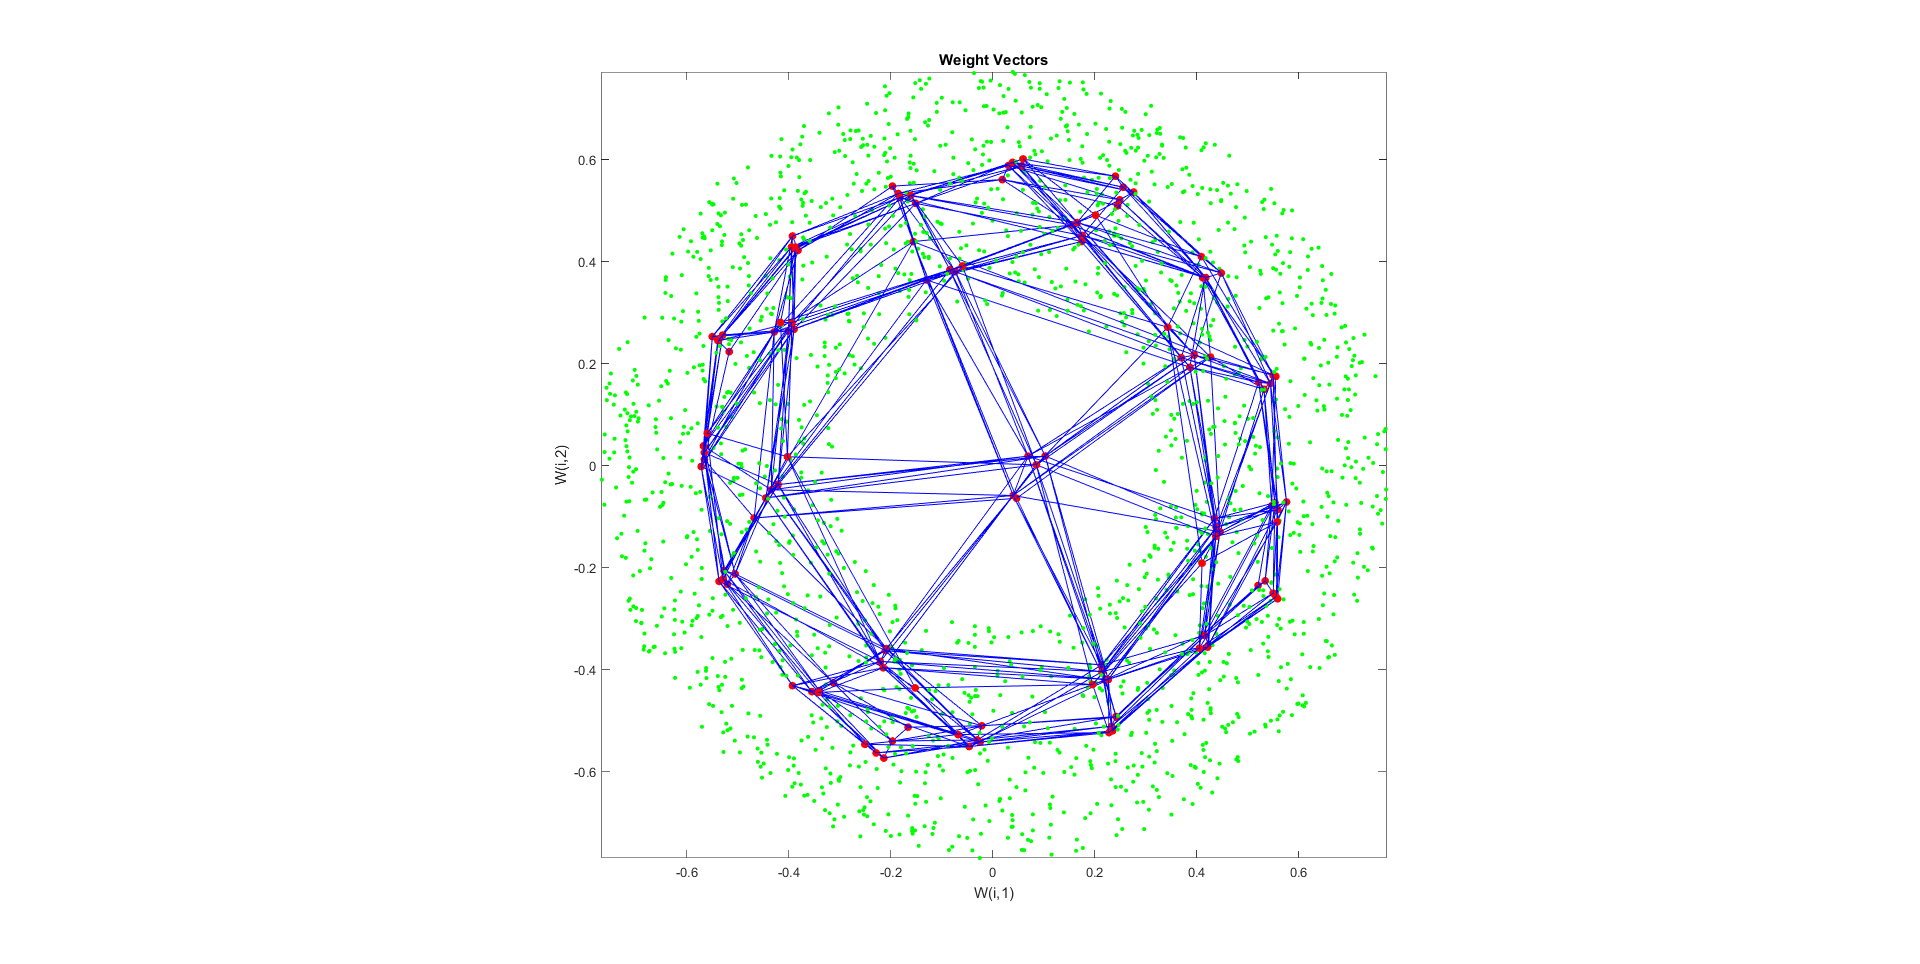
\includegraphics[width=\textwidth/5]{figures_3/som_100_2} &
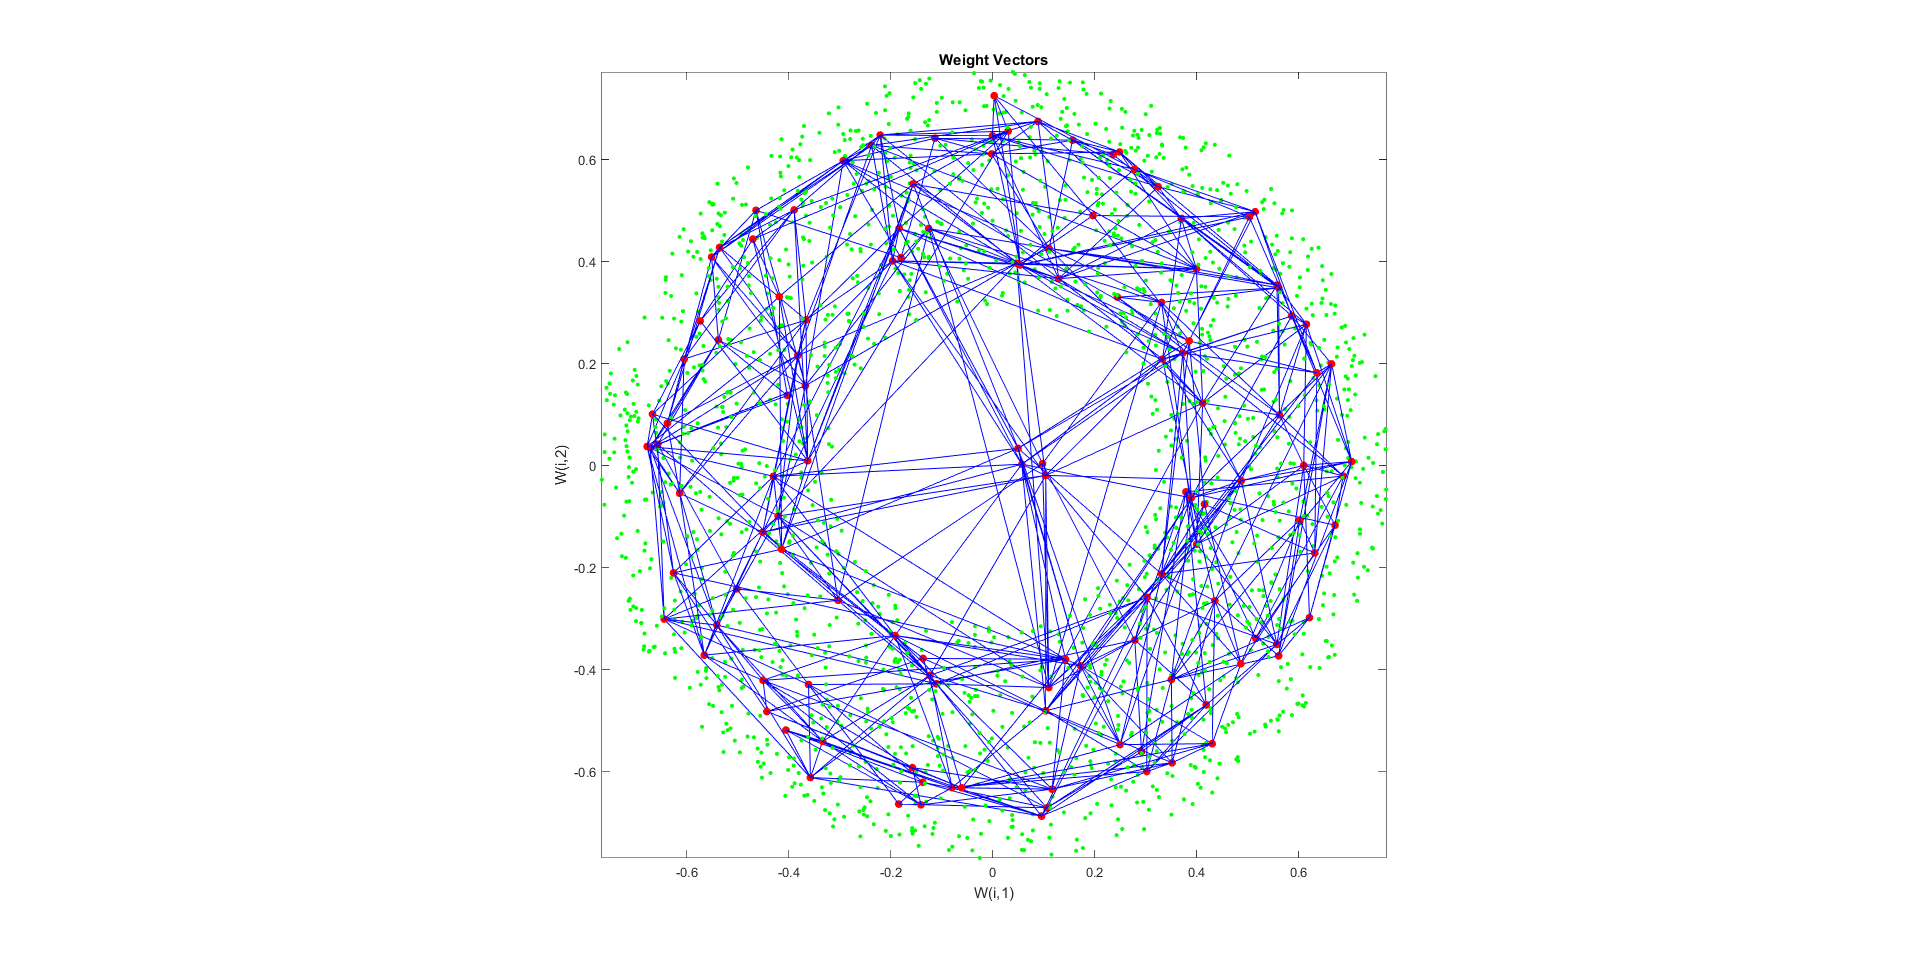
\includegraphics[width=\textwidth/5]{figures_3/som_1000_2} \\

\end{tabular}
\centering
\end{figure}

Figure \ref{panel_22} shows some results of different experiment in \textbf{example\_SOM\_iris.m} script. The model used different topologies and grid size of 10x10. \textit{Link distance} (linkdist) and \textit{Manhattan distance} (mandist) were tested with equal amount of epochs (100).
\bigbreak
A remark conclusion is that hexagonal topology shows a smoother topology than the grid topology. Additionally \textit{linkdist} gives harder limits on the decision surface than \textit{mandist} as shown in figure \ref{panel_22}.

\begin{figure}[!htbp]
\caption{Top: Plots of SOM using grid topology and \textit{linkdist}. Middle: Plots of SOM using hexagonal topology and \textit{linkdist}. Bottom: Plots of SOM using hexagonal topology and \textit{mandist}.}
\label{panel_22}
\medbreak
\begin{tabular}{ccc}
 
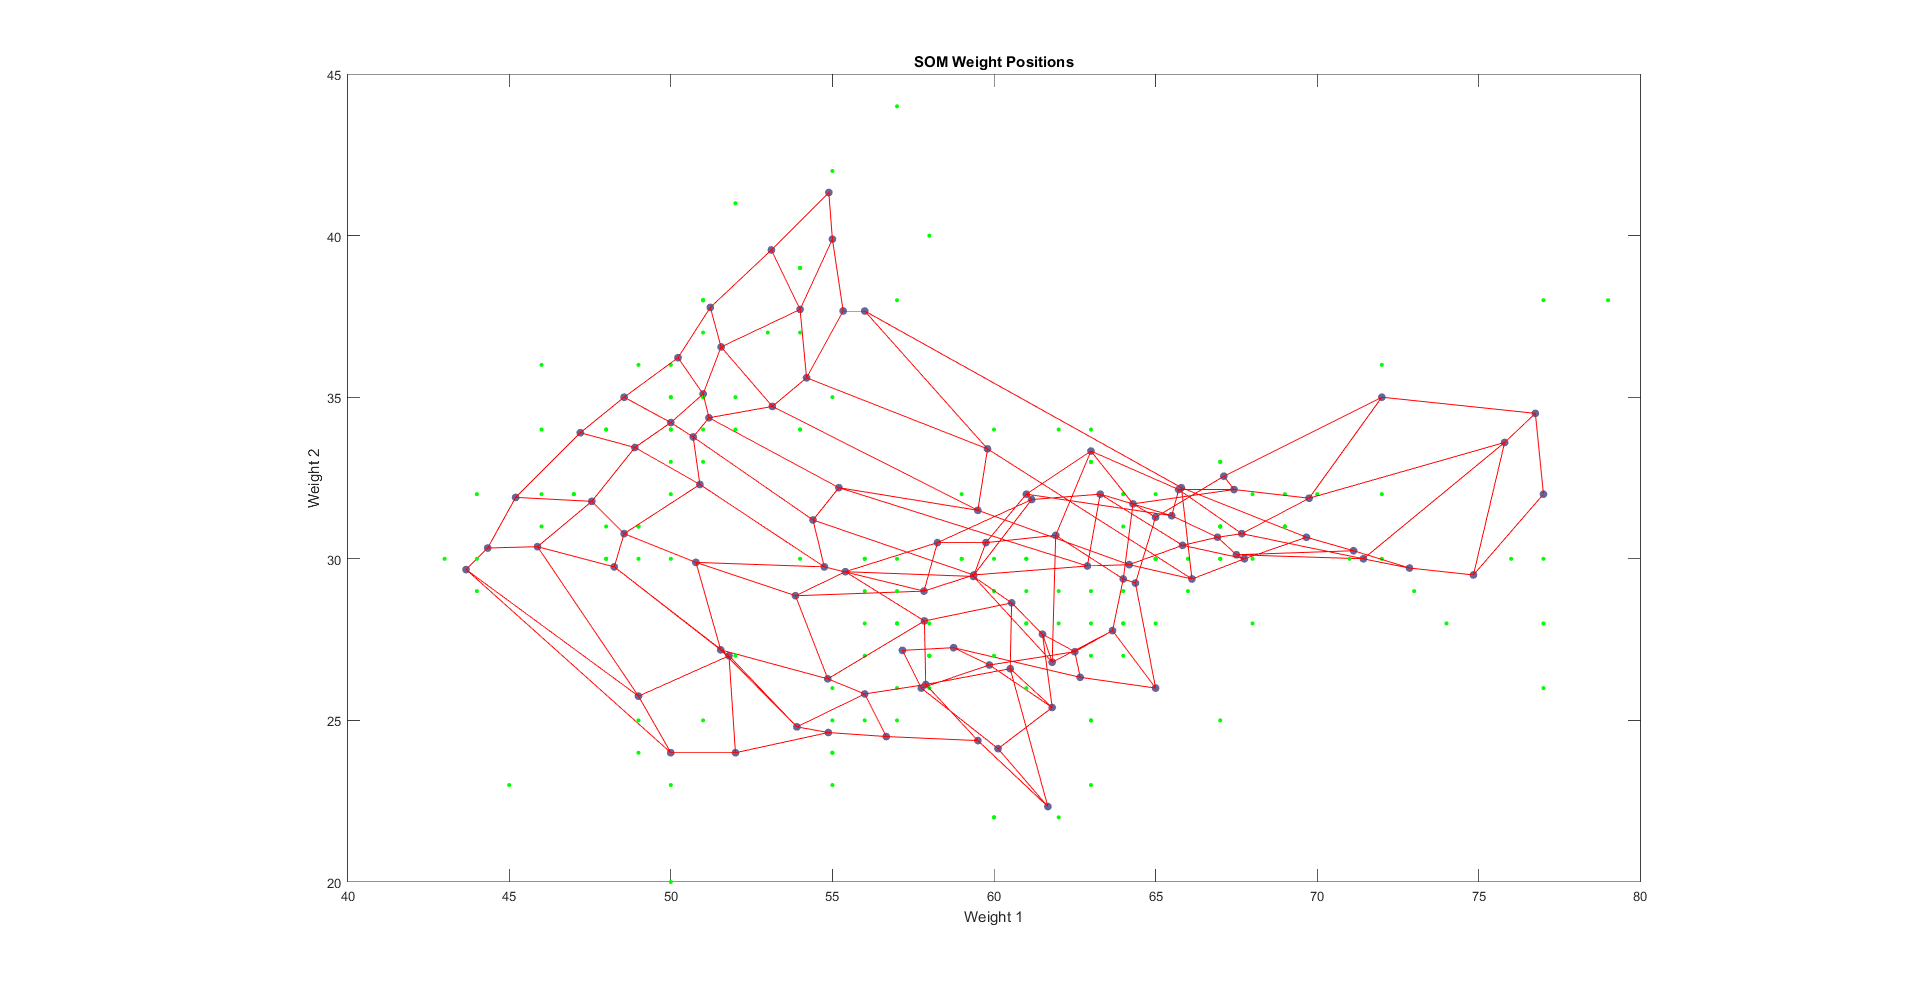
\includegraphics[width=\textwidth/4]{figures_3/som_wp_1} &
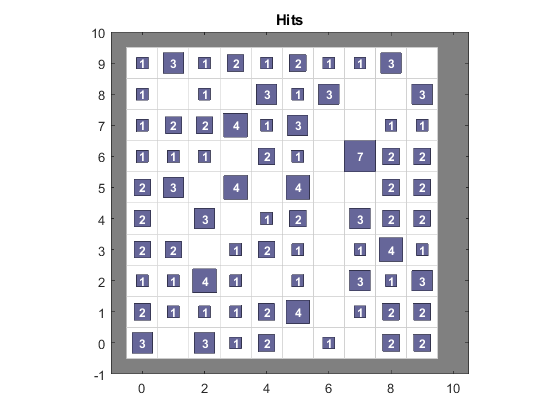
\includegraphics[width=\textwidth/5]{figures_3/som_hits_1} &
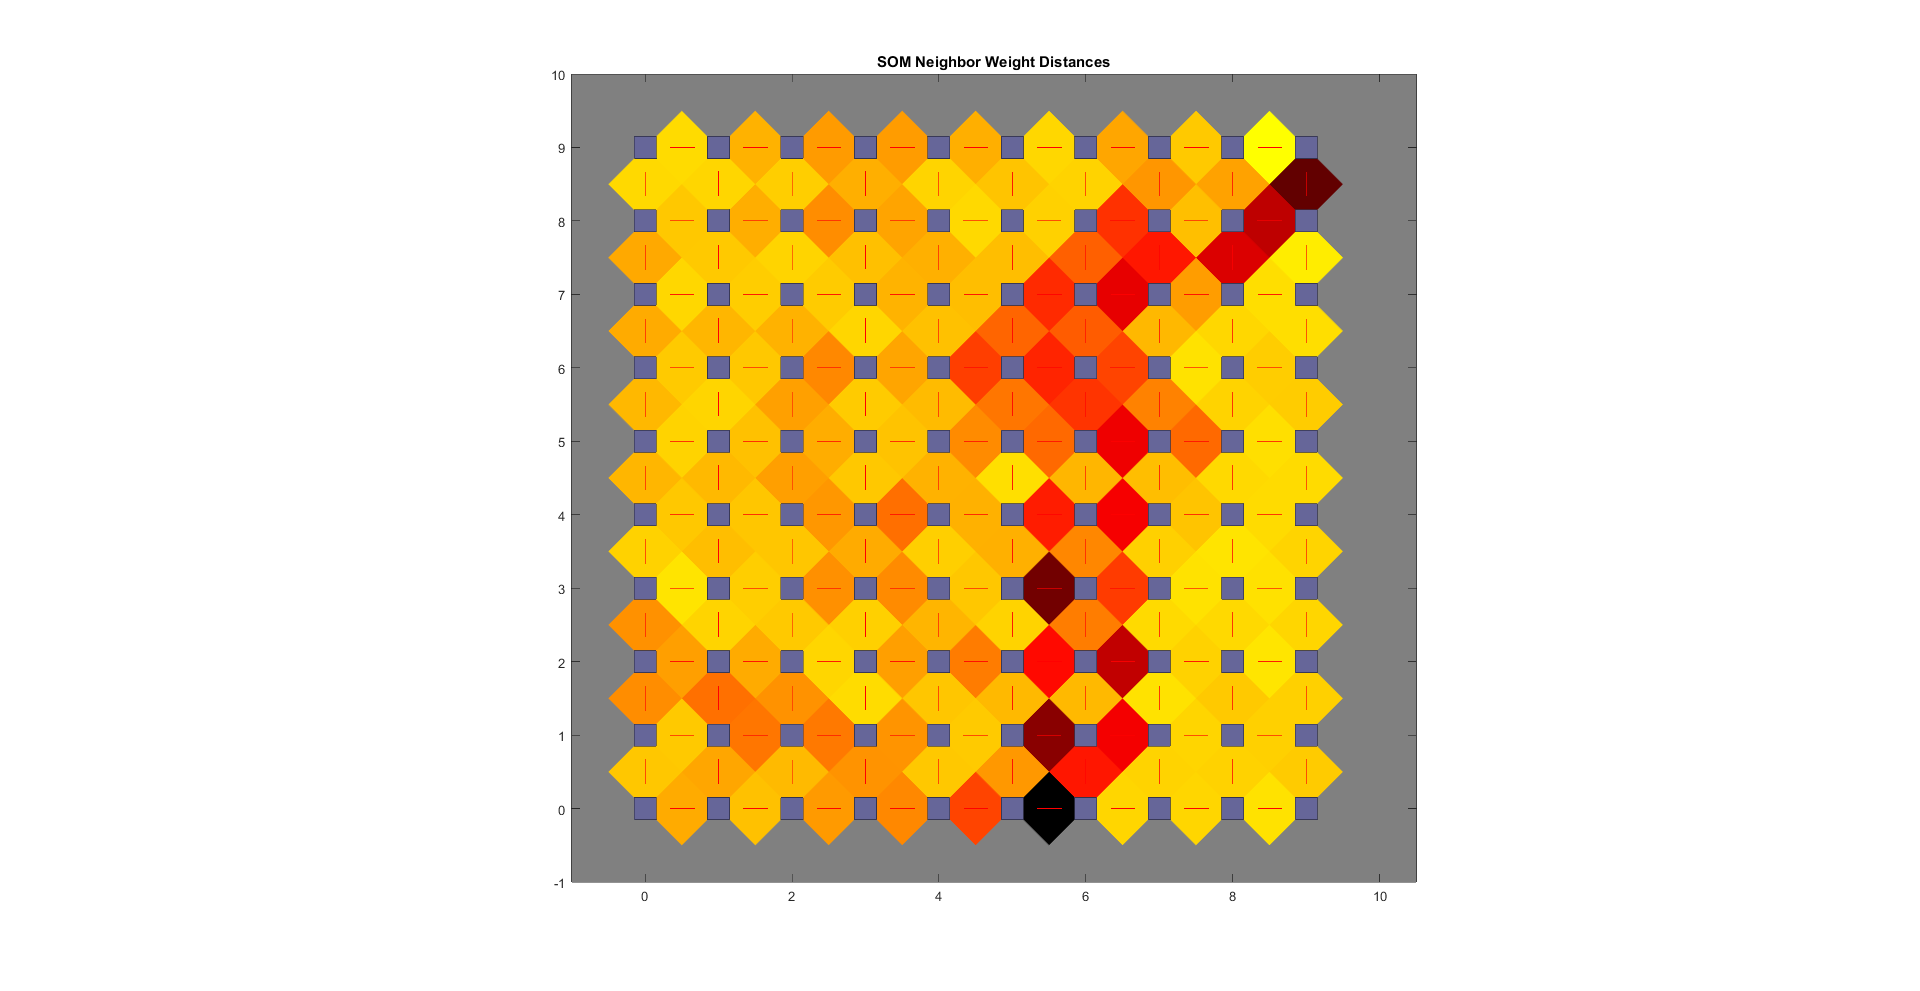
\includegraphics[width=\textwidth/4]{figures_3/som_nwd_1} \\\hline

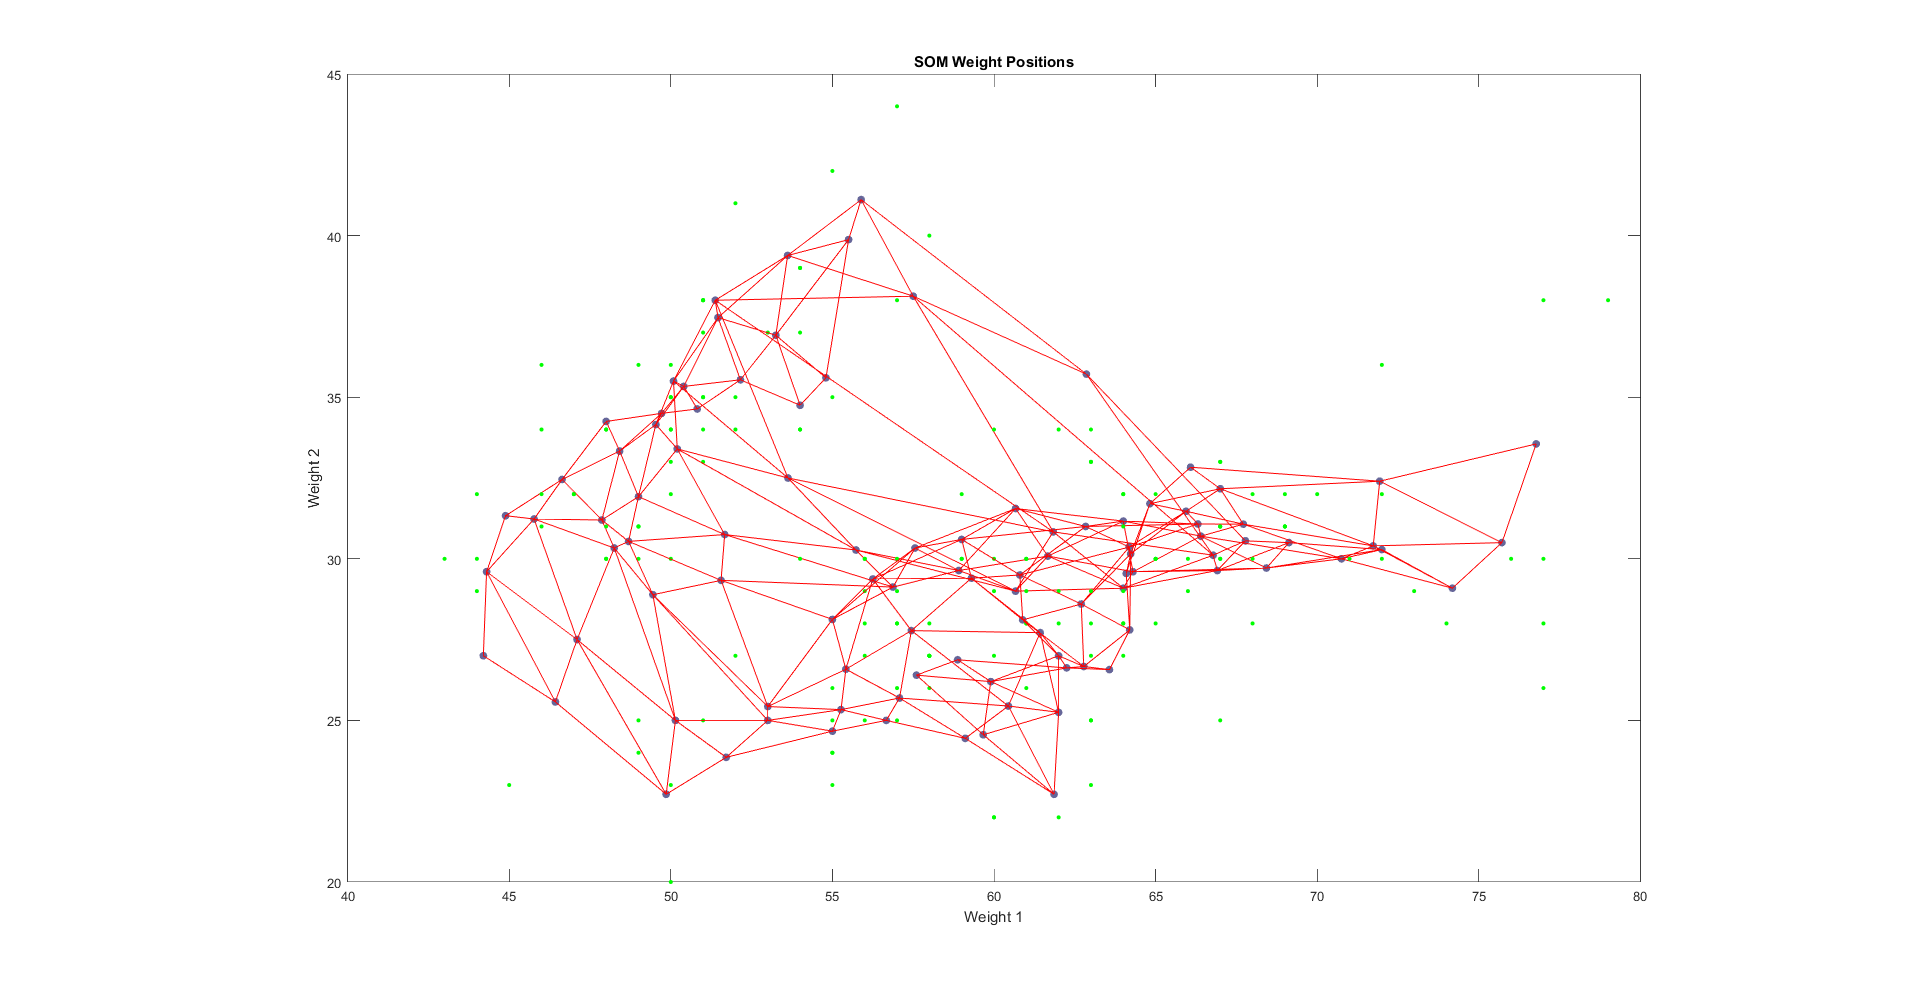
\includegraphics[width=\textwidth/4]{figures_3/som_wp_2} &
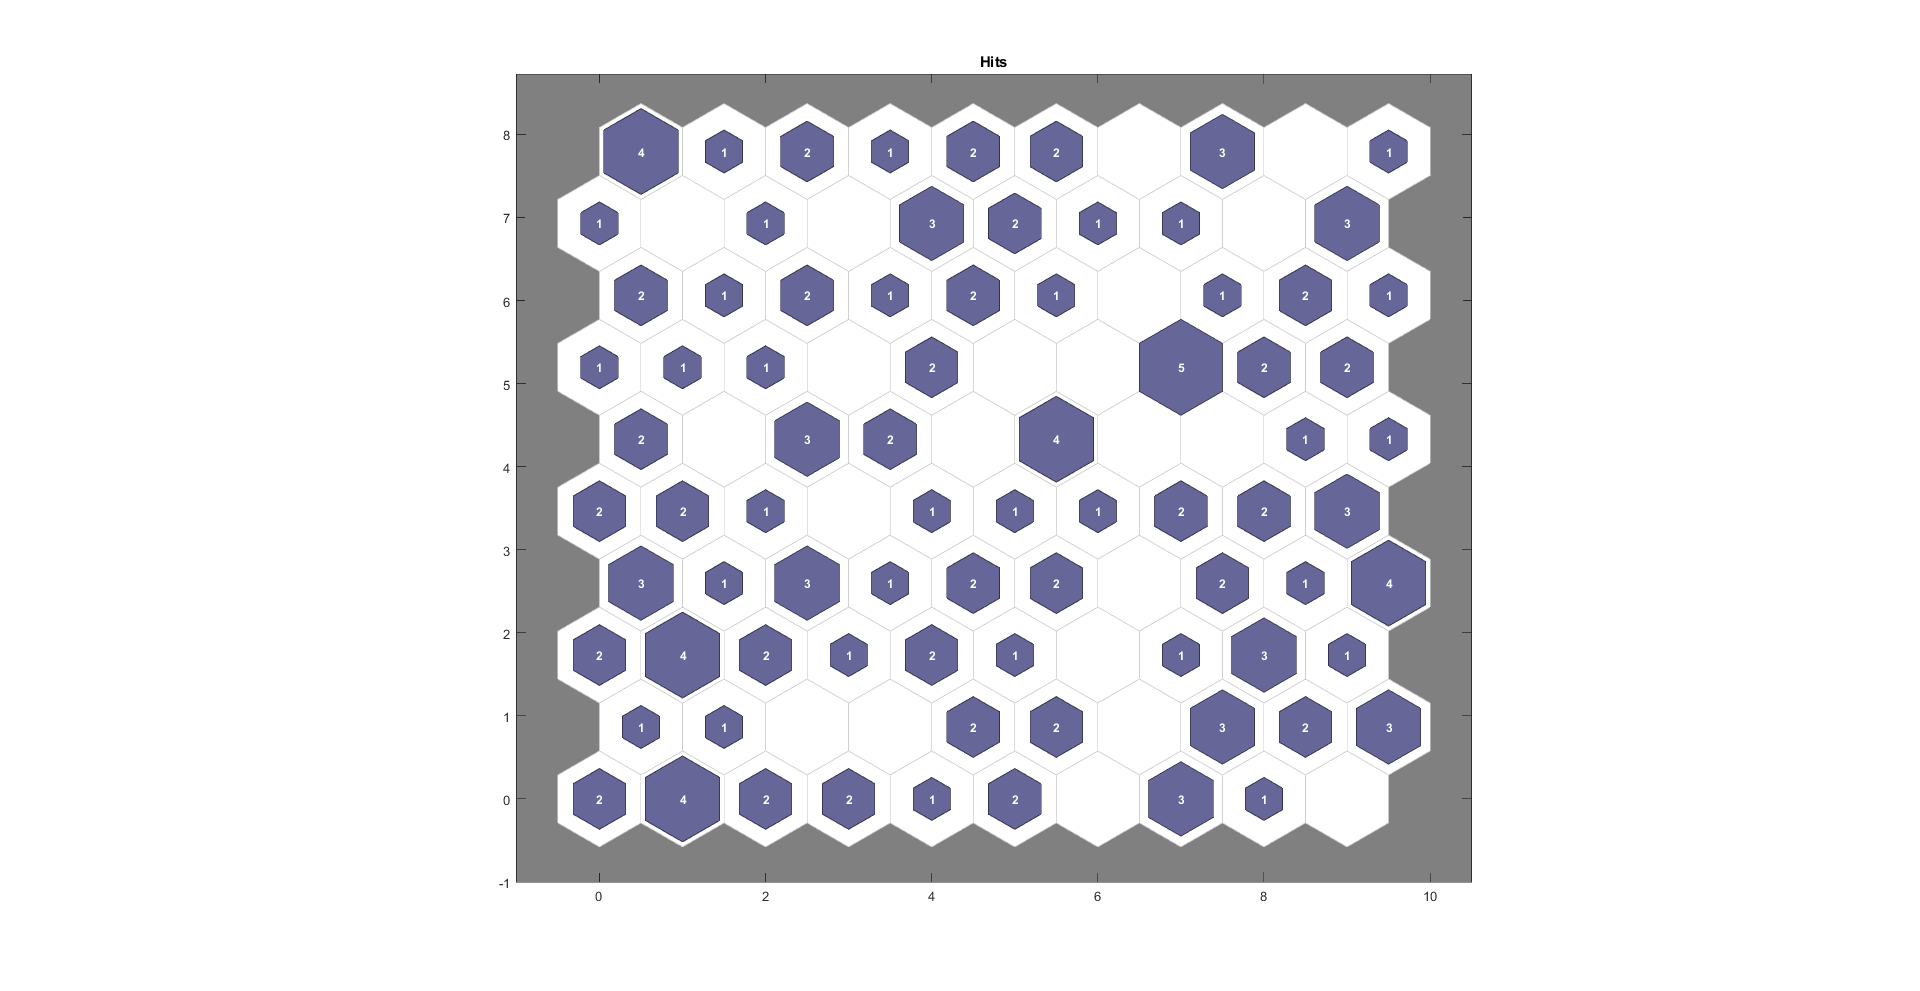
\includegraphics[width=\textwidth/4]{figures_3/som_hits_2} &
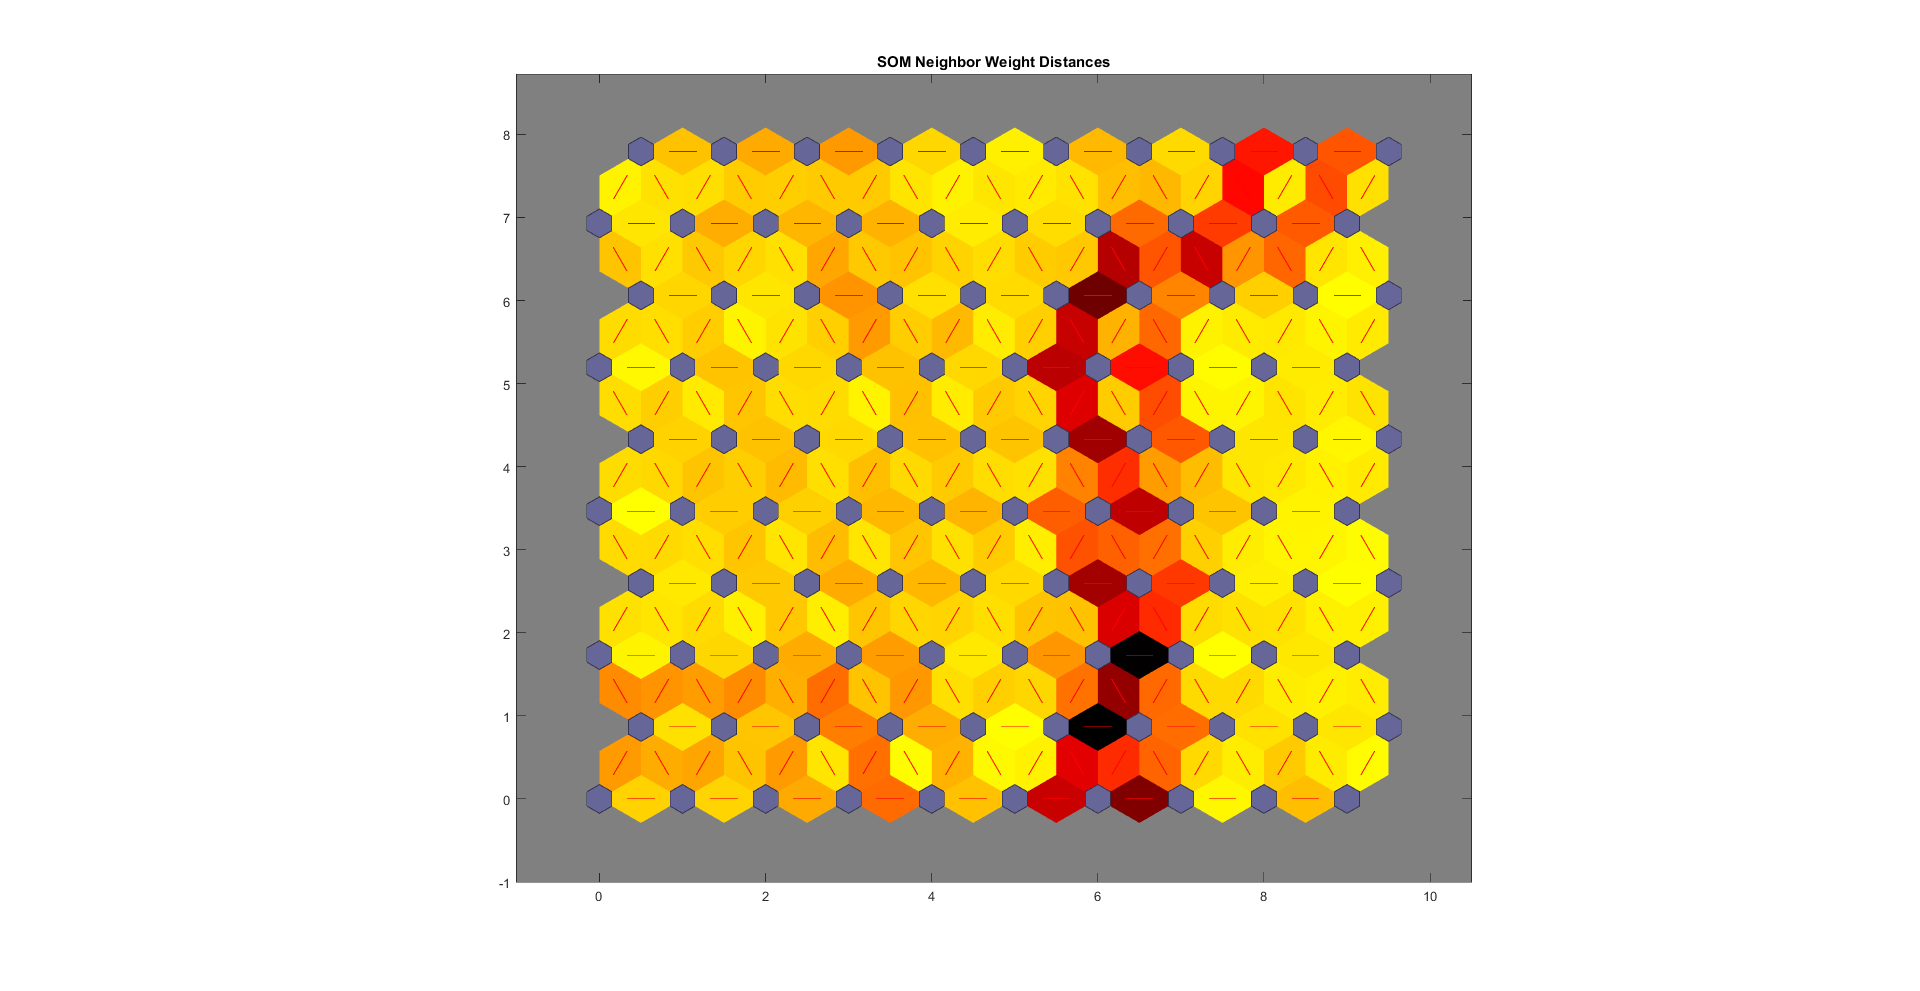
\includegraphics[width=\textwidth/4]{figures_3/som_nwd_2} \\\hline

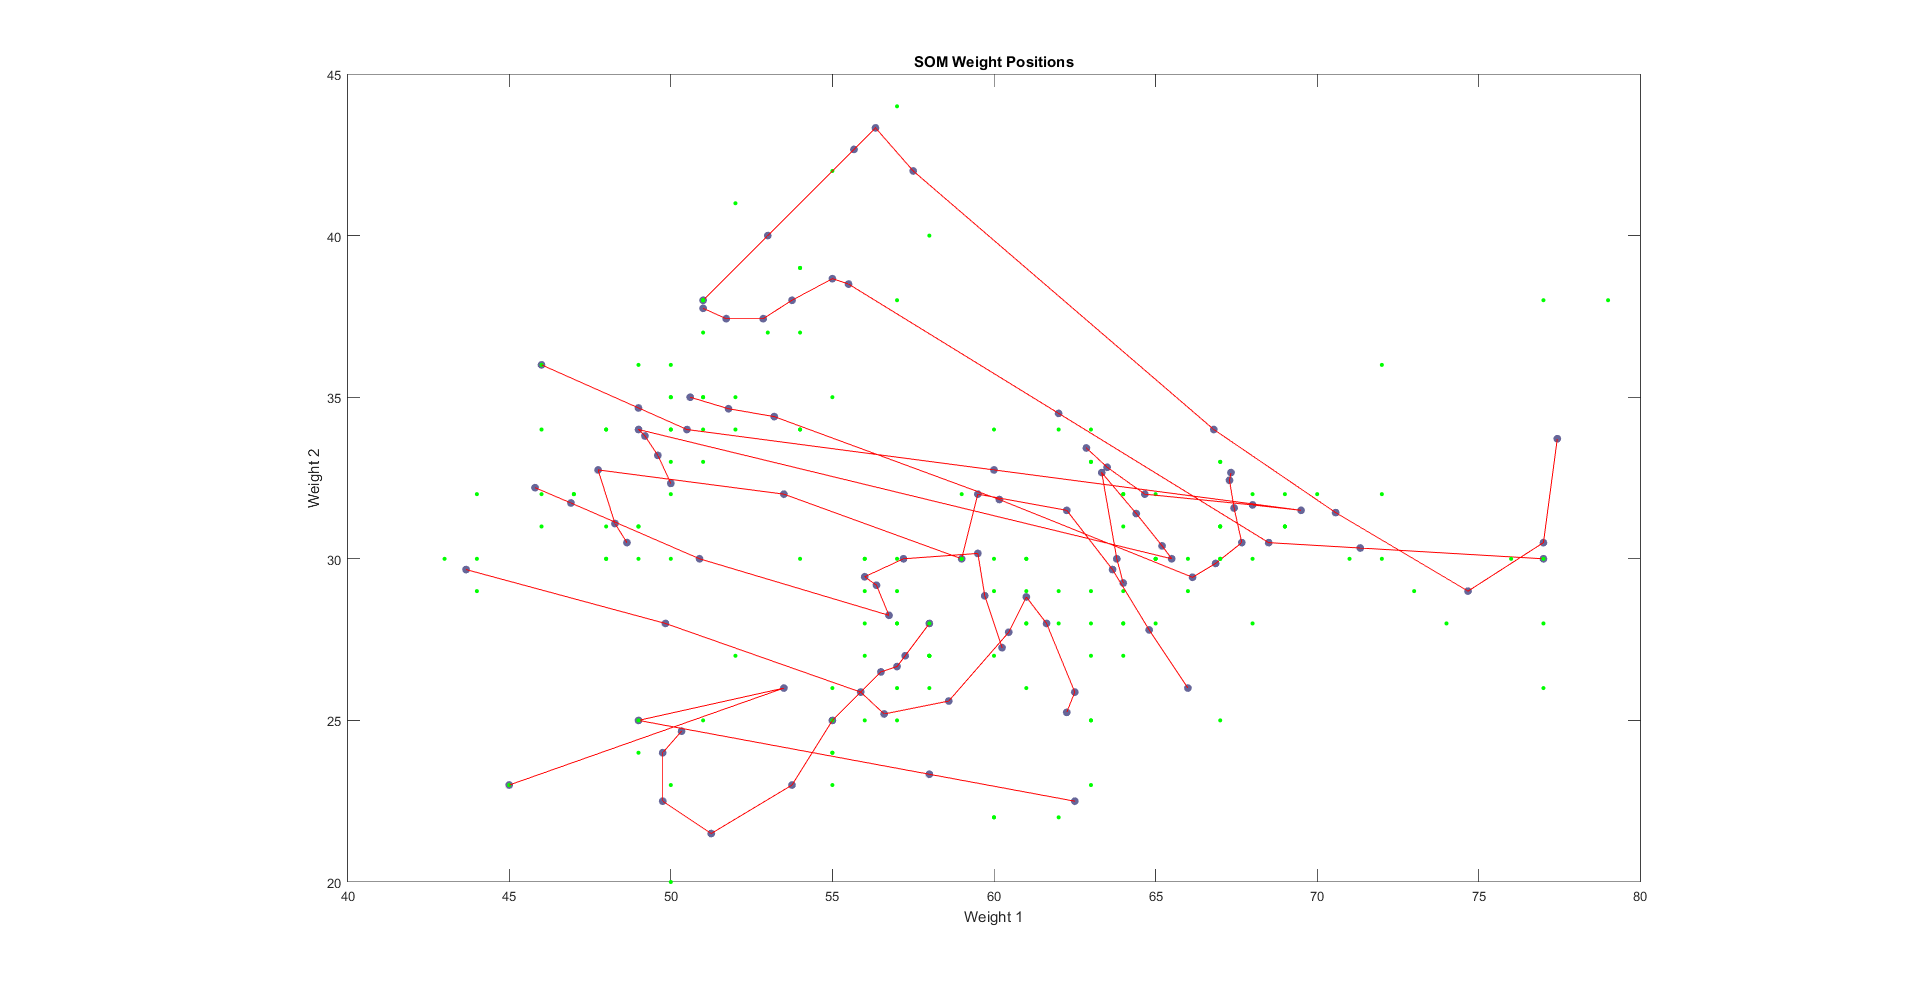
\includegraphics[width=\textwidth/4]{figures_3/som_wp_3} &
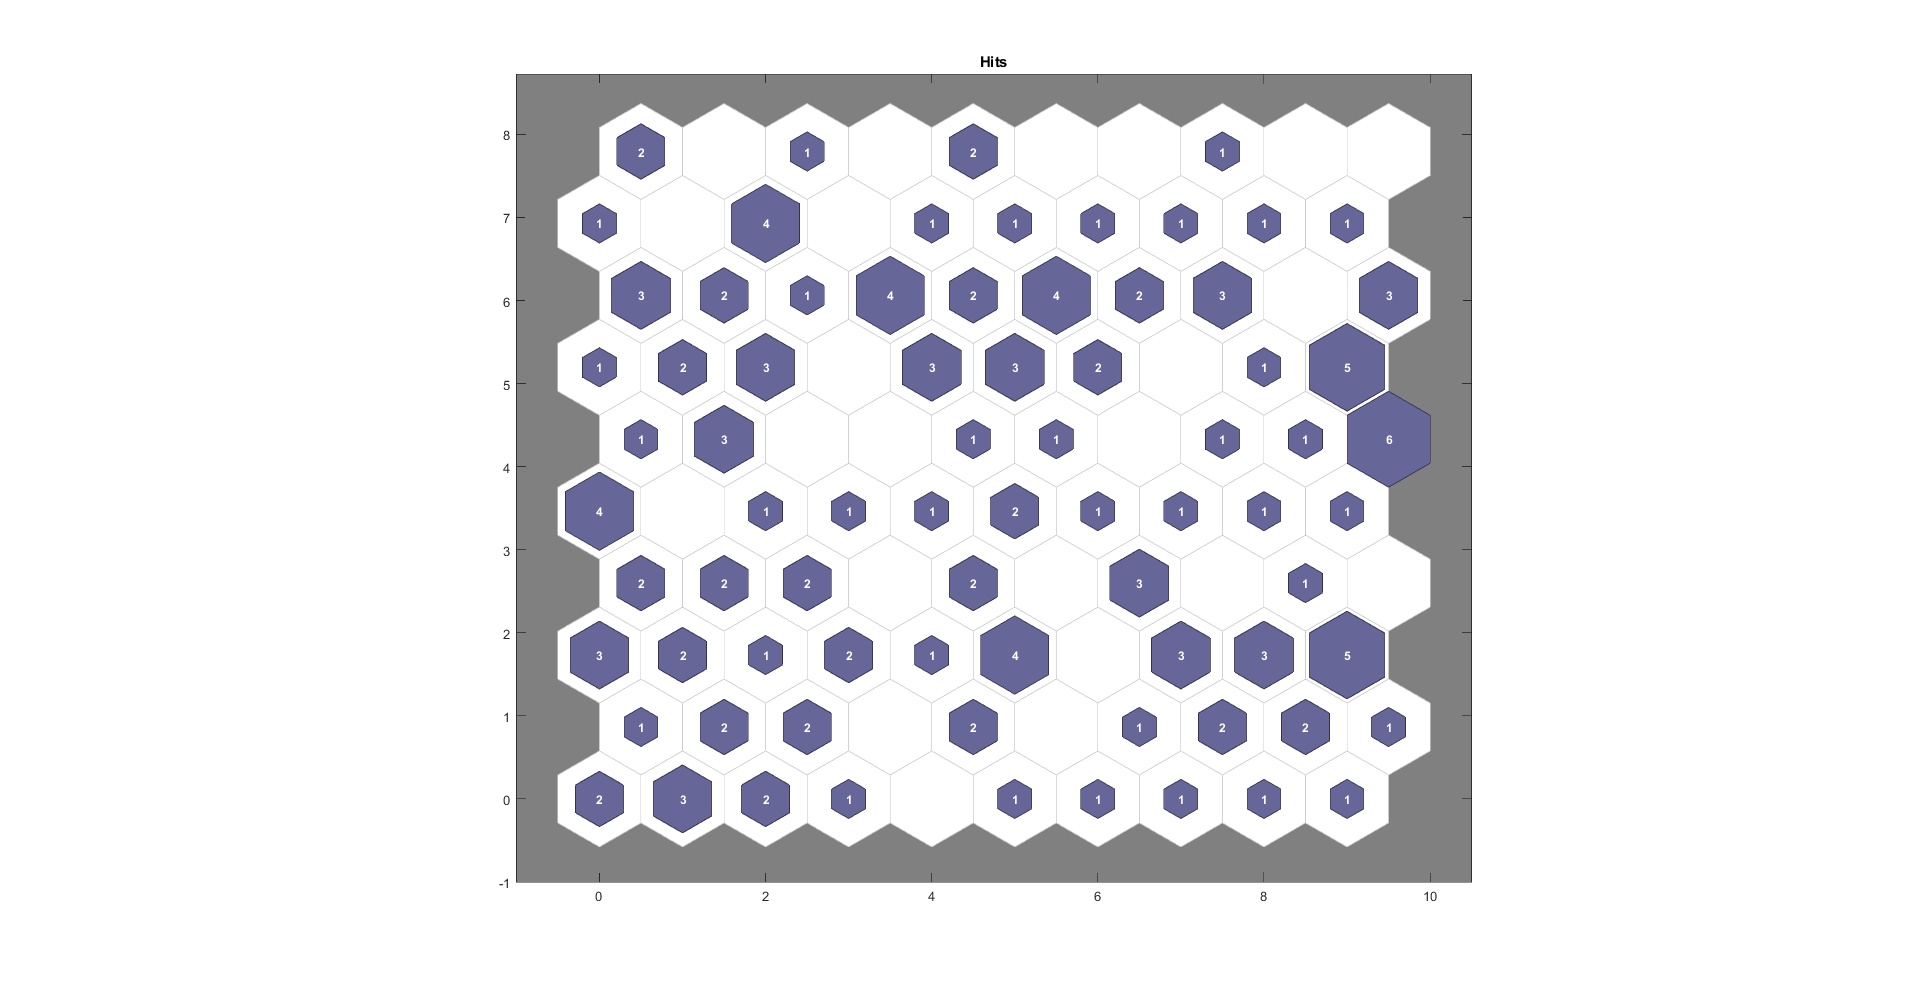
\includegraphics[width=\textwidth/4]{figures_3/som_hits_3} &
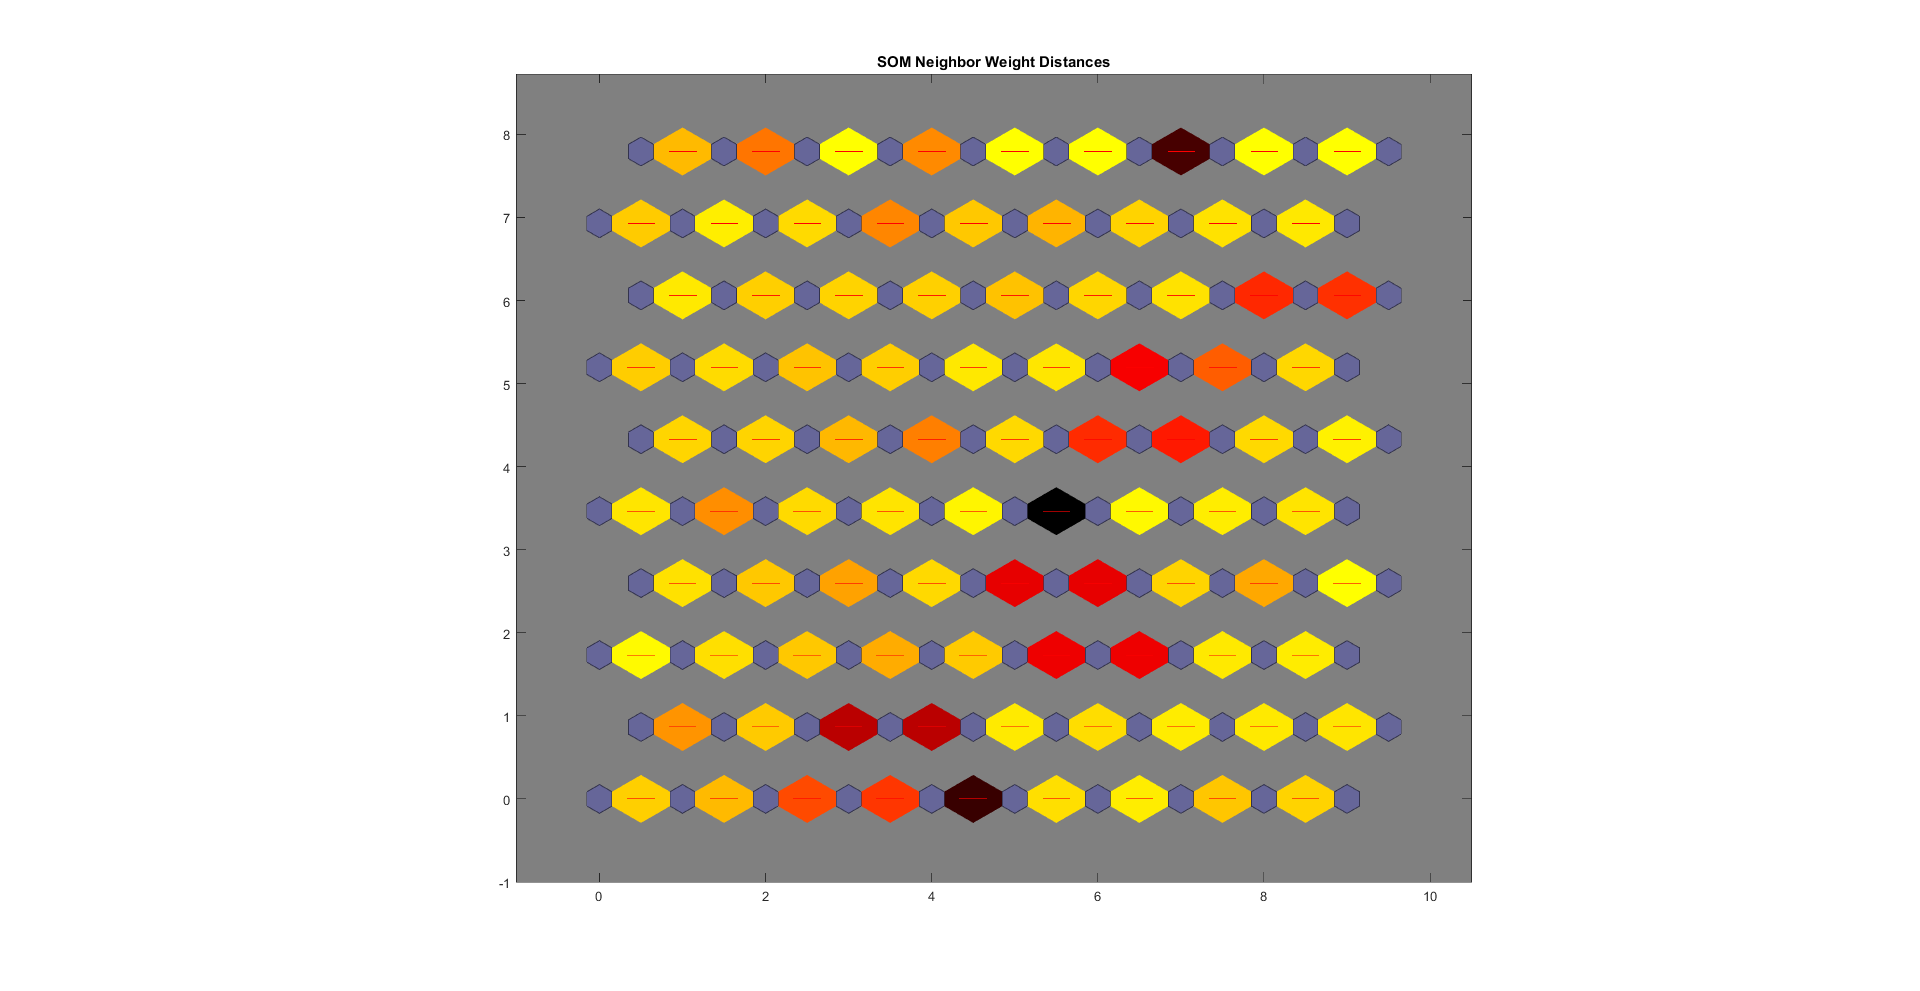
\includegraphics[width=\textwidth/4]{figures_3/som_nwd_3} \\\hline
\end{tabular}
\centering
\end{figure}